\documentclass[conference,letterpaper,10pt]{IEEEtran}
\usepackage[T1]{fontenc}
\usepackage[utf8]{inputenc}
\usepackage[spanish,es-tabla,es-nodecimaldot]{babel}
\usepackage{times,graphicx,booktabs,amsmath,amssymb,url,tabularx,array}
\usepackage[numbers]{natbib}
\usepackage{float}
\makeatletter\g@addto@macro\UrlBreaks{\do\-\do\_\do\.}\makeatother
\Urlmuskip=0mu plus 1mu
\newcommand{\rdias}{121}
\newcommand{\recoEF}{102,135}
\newcommand{\recoE}{84,956}
\newcommand{\recoF}{17,178}
\newcommand{\rbaseEF}{220,061}
\newcommand{\rbaseE}{169,276}
\newcommand{\rbaseF}{50,785}
\newcommand{\rmaEF}{57,802}
\newcommand{\rmaE}{53,774}
\newcommand{\rmaF}{4,028}
\newcommand{\recoVis}{2,263}
\newcommand{\recoBicis}{10,276}
\newcommand{\rmaVis}{2,060}
\newcommand{\rmaBicis}{10,084}
\newcommand{\rmaPct}{43.4}
\newcommand{\rmaPctLo}{41.2}
\newcommand{\rmaPctHi}{45.6}
\newcommand{\rlgbmDPct}{43.0}
\newcommand{\rlgbmDEF}{58,187}
\newcommand{\rlgbmDirPct}{43.7}
\newcommand{\rlgbmDirEF}{57,510}
\newcommand{\rorDPct}{60.0}
\newcommand{\rorDEF}{40,872}
\newcommand{\rorDirPct}{67.0}
\newcommand{\rorDirEF}{33,684}
\newcommand{\rmaGana}{121}
\newcommand{\rmaVisPct}{9.0}
\newcommand{\rmaGap}{16,930}
\newcommand{\rlgbmDirGap}{23,826}
\newcommand{\roracleDirectGap}{7,187}
\newcommand{\rmaDesvSal}{3,395}
\newcommand{\rmaDesvLleg}{311}
\newcommand{\rmaKm}{0.25}
\newcommand{\recoDesv}{2,298}
\newcommand{\recoKm}{0.26}
\newcommand{\recoNeto}{51.3}
\newcommand{\rdicPct}{39.2}
\newcommand{\rdicDias}{31}
\newcommand{\rdicMes}{diciembre de 2025}
\newcommand{\rdecTot}{44,770}
\newcommand{\rdecPNoventaCinco}{0.1}
\newcommand{\rnDiario}{4}
\newcommand{\rnDirecto}{4}
\newcommand{\rselDias}{31}
\newcommand{\rlamMa}{58.2}
\newcommand{\rlamLgbmD}{59.2}
\newcommand{\rlamLgbmDir}{68.9}
\newcommand{\rlamOrD}{44.6}
\newcommand{\rlamOrDir}{36.3}
\newcommand{\rlamDifMax}{0.89}
\newcommand{\rlamRondasMax}{4}
\newcommand{\rlamExtension}{0}
\newcommand{\rlamGridMin}{10}
\newcommand{\rlamGridMax}{120}
\newcommand{\rlamGrid}{10, 15, 20, 30, 45, 60, 75, 90, 120}
\newcommand{\rmejorReal}{media móvil}
\newcommand{\rselEcoVis}{2,033.9}
\newcommand{\rselMaVis}{2,051.5}
\newcommand{\rtopeVis}{55}
\newcommand{\rtopeBicis}{17}
\newcommand{\rpickMin}{15}
\newcommand{\rdelMin}{60}
\newcommand{\rstepMin}{15}
\newcommand{\rlagS}{30}
\newcommand{\rcovMin}{90}
\newcommand{\rtransMin}{45}
\newcommand{\rentregaCorta}{45}
\newcommand{\rentregaLarga}{75}
\newcommand{\rventanaHoras}{19.5}
\newcommand{\rabiertaPct}{95}
\newcommand{\rrefDias}{15}
\newcommand{\rnMax}{6}
\newcommand{\rlamGridN}{15, 30, 60}
\newcommand{\rtrainMeses}{8}
\newcommand{\rcurvaDias}{121}
\newcommand{\rsemanasHist}{4}
\newcommand{\rcadaTicks}{12}
\newcommand{\rlgbArboles}{200}
\newcommand{\rlgbTasa}{0.05}
\newcommand{\rlgbHojas}{31}
\newcommand{\rlgbMinHoja}{50}
\newcommand{\rlgbFilas}{0.8}
\newcommand{\rlgbCols}{0.9}
\newcommand{\rviajes}{18,689,701}
\newcommand{\rdatosPeriodo}{enero y noviembre de 2025}
\newcommand{\rviajesDia}{55,957}
\newcommand{\restaciones}{677}
\newcommand{\rbicisDistintas}{7,966}
\newcommand{\rdurMed}{12}
\newcommand{\rdurP}{37}
\newcommand{\rhuecoMed}{15.9}
\newcommand{\rhuecoTarde}{35.6}
\newcommand{\rhuecoResto}{15.3}
\newcommand{\rcalleMed}{5.3}
\newcommand{\rpicoMed}{24}
\newcommand{\rpicoNoventa}{44}
\newcommand{\rpicoNN}{61}
\newcommand{\rvDias}{121}
\newcommand{\rvEobs}{87,470}
\newcommand{\rvFobs}{17,062}
\newcommand{\rvErep}{84,956}
\newcommand{\rvFrep}{17,178}
\newcommand{\rvRel}{3}
\newcommand{\rvRelF}{-1}
\newcommand{\rsCuarenta}{$-$6,559}
\newcommand{\rsCuarentaLo}{$-$7,042}
\newcommand{\rsCuarentaHi}{$-$6,076}
\newcommand{\rsCuarentaOr}{$-$3,906}
\newcommand{\rsSetenta}{$+$6,922}
\newcommand{\rsSetentaLo}{$+$6,348}
\newcommand{\rsSetentaHi}{$+$7,496}
\newcommand{\rsSetentaOr}{$+$3,476}
\newcommand{\rsDan}{$+$1,253}
\newcommand{\rsDanLo}{$+$952}
\newcommand{\rsDanHi}{$+$1,554}
\newcommand{\rsDanOr}{$+$89}
\newcommand{\rsSinRegla}{4,615}
\newcommand{\rsSoloUno}{2,470}
\newcommand{\rsEcoEF}{102,135}
\newcommand{\rmaeMes}{septiembre de 2025}
\newcommand{\rmaeMa}{1.62}
\newcommand{\rmaeMaW}{0.81}
\newcommand{\rmaeLgbmD}{1.61}
\newcommand{\rmaeLgbmDW}{0.81}
\newcommand{\rmaeLgbmDir}{1.99}
\newcommand{\rmaeLgbmDirW}{0.88}
\newcommand{\rantPeriodo}{enero a agosto de 2025}
\newcommand{\rvisSinRegla}{5,113.5}
\newcommand{\rvisConRegla}{2,491.5}
\newcommand{\rvisQuedan}{48.7}
\newcommand{\rpruebaPeriodo}{septiembre a diciembre de 2025}
\newcommand{\rselMes}{agosto de 2025}
\newcommand{\rrefPeriodo}{septiembre a noviembre de 2025}
\newcommand{\retiquetasDia}{5,000}
\newcommand{\renSitioPct}{78}
\newcommand{\rfdFeedE}{87,470}
\newcommand{\rfdFeedF}{17,062}
\newcommand{\rfdFeedEF}{104,532}
\newcommand{\rfdSalidasDia}{52,243}
\newcommand{\recoDesvPct}{4.4}
\newcommand{\rmaDesvPct}{7.1}
\newcommand{\rorDirDesvPct}{3.6}
\newcommand{\rlgbmDirDesvPct}{7.5}
\newcommand{\rbaseDesvPct}{27.0}
\newcommand{\rfdEcoDesv}{2,298}
\newcommand{\rcfDias}{16}
\newcommand{\rcfPrimero}{1 de septiembre de 2025}
\newcommand{\rcfUltimo}{31 de diciembre de 2025}
\newcommand{\rcfSalidas}{856,176}
\newcommand{\rcfEcoDesv}{38,825}
\newcommand{\rcfEcoPct}{4.53}
\newcommand{\rcUnoSal}{22}
\newcommand{\rcUnoLle}{35}
\newcommand{\rcUnoTSal}{4.6}
\newcommand{\rcUnoTLle}{5.3}
\newcommand{\rcDosPct}{5.2}
\newcommand{\rcDosMin}{1.3}
\newcommand{\rcDosMax}{8.2}
\newcommand{\rcDosNR}{83}
\newcommand{\rcDosEdad}{12.3}
\newcommand{\rcDosSalidas}{855,867}
\newcommand{\rcTresEst}{677}
\newcommand{\rcTresSiete}{22}
\newcommand{\rcTresDoce}{149}
\newcommand{\rcTresPico}{242}
\newcommand{\rcTresPicoHora}{22:00}
\newcommand{\rcTresPicoDif}{0.9}
\newcommand{\rcTresCrudoMin}{84}
\newcommand{\rcTresCrudoMax}{496}
\newcommand{\rcTresCrudoDifMax}{2.2}
\newcommand{\rdTop}{68}
\newcommand{\rdEst}{677}
\newcommand{\rdTopViajes}{25}
\newcommand{\rdPicoHoras}{08:00--08:59 y 14:00--18:59}
\newcommand{\rdPicoSal}{45}
\newcommand{\rdEFTopEco}{9,151}
\newcommand{\rdEFTopMa}{8,278}
\newcommand{\rdEFRestoEco}{93,901}
\newcommand{\rdEFRestoMa}{50,340}
\newcommand{\rdETopEco}{6,780}
\newcommand{\rdETopMa}{7,489}
\newcommand{\rdEFTopRed}{10}
\newcommand{\rdEFRestoRed}{46}
\newcommand{\rdMaExtra}{1,611}
\newcommand{\rdMaExtraTop}{42}
\newcommand{\rdMaExtraPico}{60}
\newcommand{\rdEcoPico}{47}
\newcommand{\rdLgbmExtraTopMin}{39}
\newcommand{\rdLgbmExtraTopMax}{41}
\newcommand{\rejEst}{273-274}
\newcommand{\rejNombre}{Luis Donaldo Colosio -- Jesús García}
\newcommand{\rejDia}{1 de septiembre de 2025}
\newcommand{\rejDesde}{08:45}
\newcommand{\rejHasta}{09:00}
\newcommand{\rejFotoA}{1}
\newcommand{\rejFotoAHora}{08:36}
\newcommand{\rejFotoB}{0}
\newcommand{\rejFotoBHora}{08:48}
\newcommand{\rejFotoC}{30}
\newcommand{\rejFotoCHora}{09:06}
\newcommand{\rejMovA}{19}
\newcommand{\rejMovAHora}{08:36}
\newcommand{\rejMovB}{79}
\newcommand{\rejMovBHora}{09:06}
\newcommand{\rejMovCincuenta}{10}
\newcommand{\rejMovCuarenta}{11}
\newcommand{\rejMovVecHora}{08:48}
\newcommand{\rejSal}{40}
\newcommand{\rejDesv}{41}
\newcommand{\rejDosN}{9}
\newcommand{\rejDosM}{220}
\newcommand{\rejCincoN}{6}
\newcommand{\rejCincoM}{301}
\newcommand{\rejCuatroN}{3}
\newcommand{\rejCuatroM}{591}
\newcommand{\rejCeroN}{7}
\newcommand{\rejCeroM}{907}
\newcommand{\rejVecIni}{21}
\newcommand{\rejVecFin}{0}
\newcommand{\rejNVec}{13}
\newcommand{\rfigPeriodo}{septiembre a noviembre de 2025}
\newcommand{\rfigVisitas}{210,974}
\newcommand{\rfigBajoTope}{97.0}
\newcommand{\rfigIntervalos}{6,051}
\newcommand{\rfigVisBajoTope}{87.8}

% Generado por report/figs/figs_caso.py. No editar a mano.
\newcommand{\cdBaseE}{229,597}
\newcommand{\cdBaseF}{59,285}
\newcommand{\cdBaseEF}{288,882}
\newcommand{\cdBaseDesv}{20,452}
\newcommand{\cdBaseKm}{426}
\newcommand{\cdBaseVis}{0}
\newcommand{\cdBaseBicis}{0}
\newcommand{\cdEcoE}{106,451}
\newcommand{\cdEcoF}{12,316}
\newcommand{\cdEcoEF}{118,767}
\newcommand{\cdEcoDesv}{3,343}
\newcommand{\cdEcoKm}{279}
\newcommand{\cdEcoVis}{2,567}
\newcommand{\cdEcoBicis}{13,829}
\newcommand{\cdLgbmE}{69,037}
\newcommand{\cdLgbmF}{2,125}
\newcommand{\cdLgbmEF}{71,162}
\newcommand{\cdLgbmDesv}{5,517}
\newcommand{\cdLgbmKm}{263}
\newcommand{\cdLgbmVis}{2,692}
\newcommand{\cdLgbmBicis}{14,265}
\newcommand{\cdMaE}{68,644}
\newcommand{\cdMaF}{1,787}
\newcommand{\cdMaEF}{70,431}
\newcommand{\cdMaDesv}{5,469}
\newcommand{\cdMaKm}{260}
\newcommand{\cdMaVis}{2,705}
\newcommand{\cdMaBicis}{13,988}
\newcommand{\cdOrE}{36,227}
\newcommand{\cdOrF}{851}
\newcommand{\cdOrEF}{37,078}
\newcommand{\cdOrDesv}{2,922}
\newcommand{\cdOrKm}{257}
\newcommand{\cdOrVis}{2,797}
\newcommand{\cdOrBicis}{12,430}
\newcommand{\cdLgbmPct}{40.1}
\newcommand{\cdEcoPct}{58.9}
\newcommand{\coRecogidas}{5,053}
\newcommand{\coFalta}{196}
\newcommand{\coFaltaPct}{3.7}
\newcommand{\coDevueltas}{22}
\newcommand{\coDevueltasPct}{0.43}
\newcommand{\cmBaseKm}{383}
\newcommand{\cmBaseDesv}{14,118}
\newcommand{\cmEcoKm}{259}
\newcommand{\cmEcoDesv}{2,298}
\newcommand{\cmLgbmKm}{248}
\newcommand{\cmLgbmDesv}{3,917}
\newcommand{\cmMaKm}{246}
\newcommand{\cmMaDesv}{3,706}
\newcommand{\csBaseNueveEF}{4,136}
\newcommand{\csBaseNueveDesv}{513}
\newcommand{\csBaseNueveAcum}{23,744}
\newcommand{\csBaseVeintiunoEF}{4,797}
\newcommand{\csBaseVeintiunoDesv}{318}
\newcommand{\csBaseVeintiunoAcum}{214,940}
\newcommand{\csEcoNueveEF}{2,880}
\newcommand{\csEcoNueveDesv}{121}
\newcommand{\csEcoNueveAcum}{20,667}
\newcommand{\csEcoVeintiunoEF}{2,140}
\newcommand{\csEcoVeintiunoDesv}{54}
\newcommand{\csEcoVeintiunoAcum}{95,824}
\newcommand{\csLgbmNueveEF}{1,812}
\newcommand{\csLgbmNueveDesv}{228}
\newcommand{\csLgbmNueveAcum}{14,386}
\newcommand{\csLgbmVeintiunoEF}{848}
\newcommand{\csLgbmVeintiunoDesv}{53}
\newcommand{\csLgbmVeintiunoAcum}{58,335}
\newcommand{\cvDiasVeinticinco}{365}
\newcommand{\cvOkVeinticinco}{351}
\newcommand{\cvExcVeinticinco}{14}
\newcommand{\cvExcJul}{12}
\newcommand{\cvDiasPrueba}{122}
\newcommand{\cvOkPrueba}{121}
\newcommand{\cvDifPrueba}{1}
\newcommand{\cvDiaExcl}{10 de septiembre}
\newcommand{\ctopeVis}{55}
\newcommand{\ctopeBicis}{17}
\newcommand{\ctopeDias}{351}
\newcommand{\ctopePeriodo}{2025}
\newcommand{\cfigVisitas}{630,433}
\newcommand{\cfigIntervalos}{23,336}
\newcommand{\cfigSinVisita}{2.1}
\newcommand{\cfigBajoTope}{95.2}
\newcommand{\cfigVisBajoTope}{94.9}
\newcommand{\cfigVisPNoventaCinco}{55.16}
\newcommand{\cfigMedBicis}{4}
\newcommand{\cfigUnaDos}{40}
\newcommand{\cfigMedVis}{20}
\newcommand{\chBicisDia}{10,276}
\newcommand{\chVisDia}{2,263}
\newcommand{\chPorQuince}{132}
\newcommand{\chVisQuince}{29}
\newcommand{\chPicoHora}{09:00}
\newcommand{\chPicoBicis}{1,009}
\newcommand{\chMananaPct}{23}
\newcommand{\chTardePct}{34}
\newcommand{\cnDias}{121}
\newcommand{\chViajesPico}{18:00}
\newcommand{\cbDias}{122}
\newcommand{\cbPares}{121}
\newcommand{\cbMedia}{-3}
\newcommand{\cbLo}{-27}
\newcommand{\cbHi}{21}
\newcommand{\cbTotMed}{7,004}
\newcommand{\cbActivasSep}{6,069}
\newcommand{\cbActivasOct}{6,119}
\newcommand{\cbActivasNov}{5,970}
\newcommand{\cbIdsNuevos}{3}
\newcommand{\cfDifDPri}{1.2}
\newcommand{\cfDifDirPri}{22.7}
\newcommand{\cfDifDUlt}{1.1}
\newcommand{\cfDifDirUlt}{22.1}
\newcommand{\cfMejorD}{si}
\newcommand{\cfMejorDir}{no}
\newcommand{\cfMeses}{4}
\newcommand{\cfMaeMaPri}{1.6}
\newcommand{\cfWapeMaSal}{40}
\newcommand{\cxEco}{102,135}
\newcommand{\cxMa}{57,802}
\newcommand{\cxMaPct}{43.4}
\newcommand{\cxDias}{121}
\newcommand{\cxCortaPct}{49.8}
\newcommand{\cxLargaPct}{36.6}
\newcommand{\cxDanPct}{42.2}

\newcommand{\caDias}{121}
\newcommand{\caAlfas}{0, 1, 3, 5, 10}
\newcommand{\caCeroKm}{4,927}
\newcommand{\caEcoKm}{3,181}
\newcommand{\caUnoKm}{24.3}
\newcommand{\caUnoEF}{0.6}
\newcommand{\caDiezKm}{50.9}
\newcommand{\caDiezEF}{6.4}
\newcommand{\caDiezEco}{39.8}
\newcommand{\caDiezBicis}{7.0}
\newcommand{\caDiezDesv}{7.0}
\newcommand{\caDiezVis}{8.9}
\newcommand{\caDiezKmEco}{23.9}
\newcommand{\caEcoEmpar}{96}

\newcommand{\rtDias}{121}
\newcommand{\rtQuinceEcoMax}{246}
\newcommand{\rtQuinceMaMax}{61}
\newcommand{\rtQuinceEcoP}{78}
\newcommand{\rtQuinceMaP}{54}
\newcommand{\rtHoraEcoP}{243}
\newcommand{\rtHoraMaP}{213}
\newcommand{\rtTresEcoMax}{1,390}
\newcommand{\rtTresMaMax}{651}
\newcommand{\rtTresBEcoP}{3,676}
\newcommand{\rtTresBMaP}{3,697}
\newcommand{\rtQuinceEcoMed}{24}
\newcommand{\rtQuinceMaMed}{24}

\renewcommand{\ttdefault}{lmtt}
\newcommand{\EF}{E+F}
\renewcommand{\IEEEkeywordsname}{Palabras clave}
\newcolumntype{Y}{>{\raggedright\arraybackslash}X}
\setcounter{dbltopnumber}{2}\renewcommand{\dbltopfraction}{0.8}
\begin{document}
\raggedbottom
\title{Pronóstico y asignación para el rebalanceo de Ecobici: un modelo de optimización bajo restricciones logísticas}
\author{\IEEEauthorblockN{Jerónimo Deli}\IEEEauthorblockA{Ciencia de Datos Aplicada, ITAM\\Ciudad de México}}
\maketitle

\begin{abstract}
La demanda de Ecobici, el sistema de bicicletas públicas de la Ciudad de México, cambia a lo largo del día: en hora pico unas estaciones se quedan sin bicis mientras otras se llenan por completo, y hoy equipos del propio sistema rebalancean durante el día para corregirlo. En este trabajo medimos ese rebalanceo con datos públicos, reconstruimos a partir de ellos su logística y la usamos como restricción de un algoritmo de asignación que, cada quince minutos y a partir de un pronóstico de viajes, decide cuántas bicis recoger y entregar en cada estación. En un mismo simulador, viaje por viaje y durante los cuatro últimos meses de 2025, comparamos el rebalanceo de Ecobici con el asignador alimentado por tres pronósticos y por información perfecta. Con un pronóstico sencillo y el mismo número de visitas que Ecobici en los días en que se ajustó, el asignador reduce casi a la mitad el tiempo con estaciones vacías o llenas; un modelo más complejo no mejora el resultado, y en las estaciones de mayor demanda la ventaja casi desaparece.
\end{abstract}
\begin{IEEEkeywords}
Ecobici, rebalanceo, bicicletas compartidas, pronóstico, algoritmo greedy, simulación.
\end{IEEEkeywords}

% ======================================================================
\section{Contexto}
La Ciudad de México mueve todos los días a millones de personas en un sistema de transporte muy fragmentado, que incluye Metro, Metrobús, RTP, microbuses y combis concesionados, bicicletas públicas, plataformas digitales y automóvil privado; en un día entre semana, la zona metropolitana suma 34.56 millones de viajes \cite{inegi2017}. Cada modo tiene su propia cobertura, costo, horario y nivel de seguridad, y no todos los habitantes tienen acceso a los mismos modos ni los usan de la misma manera \cite{caso2026}.

La información sobre esa movilidad es igual de desigual. Hay datos de afluencia del Metro y encuestas origen-destino, pero el transporte concesionado, que mueve a la mayoría de la población, opera sin un registro sistemático de rutas, tiempos o usuarios, y el resto de las fuentes, desde plataformas de navegación hasta registros de la Fiscalía, está disperso. Tampoco hay consenso entre autoridades, concesionarios y ciudadanía sobre cuál es el problema de movilidad más urgente, ni para quién \cite{caso2026}.

Ecobici es una excepción en este panorama, porque publica sus datos. Con 9,308 bicicletas es el sistema de bicicletas públicas con más unidades de América Latina, por delante de BikeSantiago y de BikeItaú en São Paulo, con 3,500 cada uno \cite{eluniversal2025semovi}, y opera unas 687 estaciones \cite{expansion2026}. En 2025 registró más de 19.4 millones de viajes de 284,289 personas \cite{ecobici2025balance}. Su principal problema es la disponibilidad: en la encuesta oficial de 2025, la desventaja que más usuarios eligieron fue que no siempre hay bicis disponibles (1,990 de 4,139 respuestas), muy por encima de la falta de espacios para anclar (114) \cite{encuesta2025}.

Al revisar la literatura y los datos disponibles, Ecobici resulta sumamente atractivo por la cantidad de datos públicos, que registran cada viaje con su bici, sus estaciones y su hora, y por la naturaleza del rebalanceo, un problema de decisión que se puede medir y donde hay mucho espacio para modelos de datos y algoritmos. La literatura lo ha abordado desde varios ángulos. Los modelos estáticos \cite{raviv2013static,dellamico2014} reacomodan el sistema de noche, con la demanda detenida, y buscan las rutas más baratas para los vehículos sobre instancias de prueba. Los dinámicos \cite{schuijbroek2017,legros2019} deciden durante el día y combinan inventarios objetivo por estación con rutas o reglas de prioridad. Otra línea pronostica las salidas y llegadas de cada estación \cite{li2015traffic} y se evalúa por su error, no por cuánto mejora el servicio. Para Ecobici, Gómez et al. \cite{gomez2021} optimizan con simulación los inventarios por estación, y Possani et al. \cite{possani2021}, el inventario junto con el ruteo. En general, estos trabajos obtienen buenos resultados frente a sus propias referencias, pero no los comparan con la logística que el operador ejecuta en la calle, de modo que su análisis no termina en algo accionable. Los trabajos que sí miran al operador real \cite{medard2016,luo2026} infieren su rebalanceo a partir de datos públicos, pero no proponen ni prueban una alternativa. Nuestro trabajo une las dos partes: medimos lo que hace Ecobici con sus propios datos y, en el mismo simulador, con los mismos viajes y con una logística comparable, lo enfrentamos a políticas que pronostican y asignan.

% ======================================================================
\section{Definición del problema}
\subsection{La demanda dinámica}
Reconocemos que la demanda dinámica es la principal causa de que las bicicletas queden mal colocadas. Las actividades diarias de la gente trazan una ruta natural: en la mañana las estaciones cercanas a las oficinas se saturan mientras las zonas residenciales se vacían, y en la noche ocurre lo contrario. La Fig.~\ref{fig:sin} muestra este patrón el lunes \rejDia. A las 9:00 las estaciones de oficinas sobre Reforma están llenas y las del norte, vacías; a las 21:00 se vacía Polanco y se llena parte del norte.

\begin{figure}[!htb]
\centering
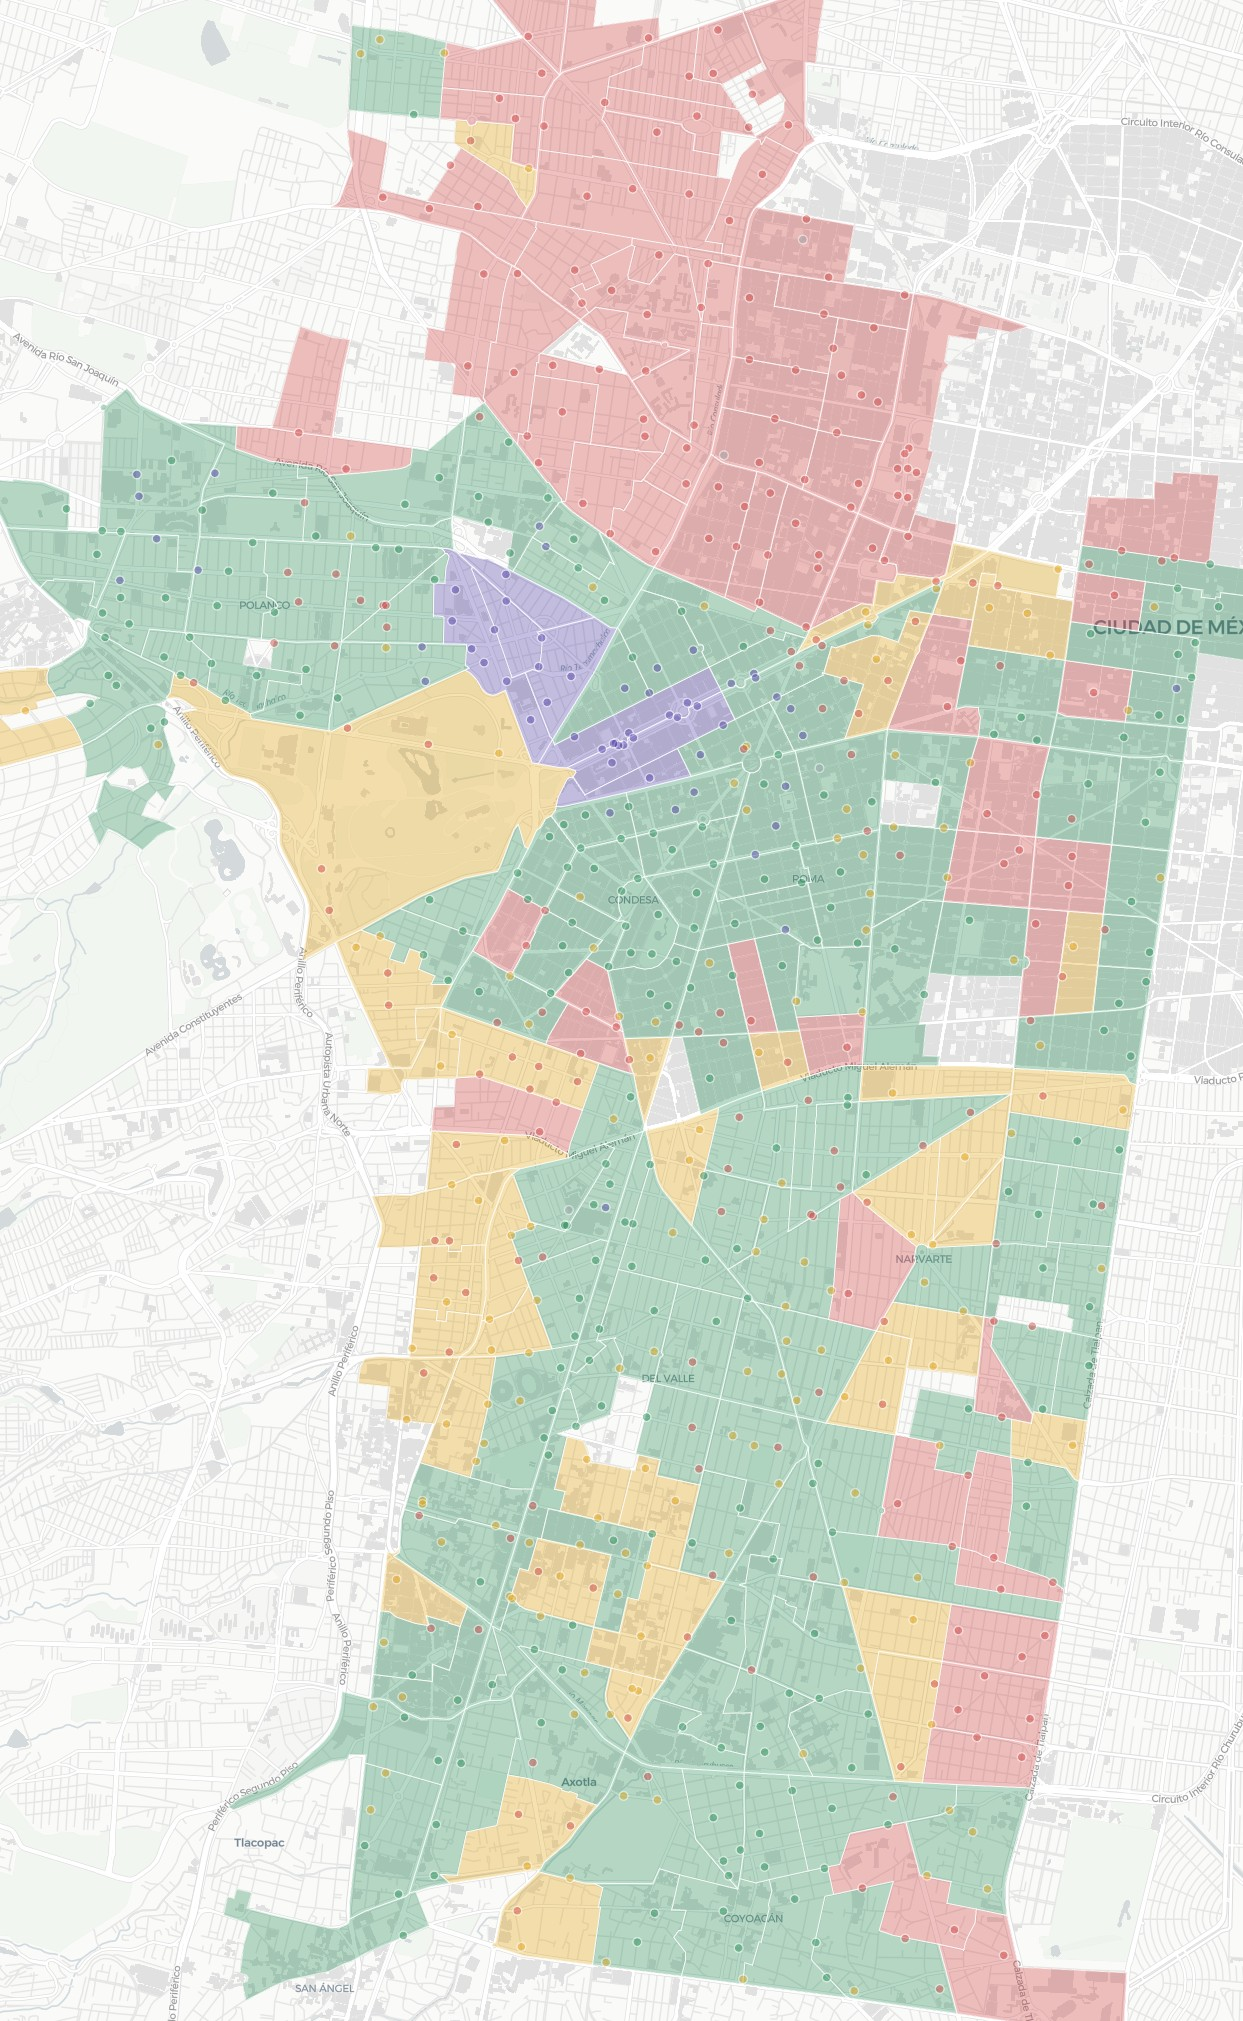
\includegraphics[height=2.1in]{figs/app-caso/sin-0900-col.jpg}\hfill
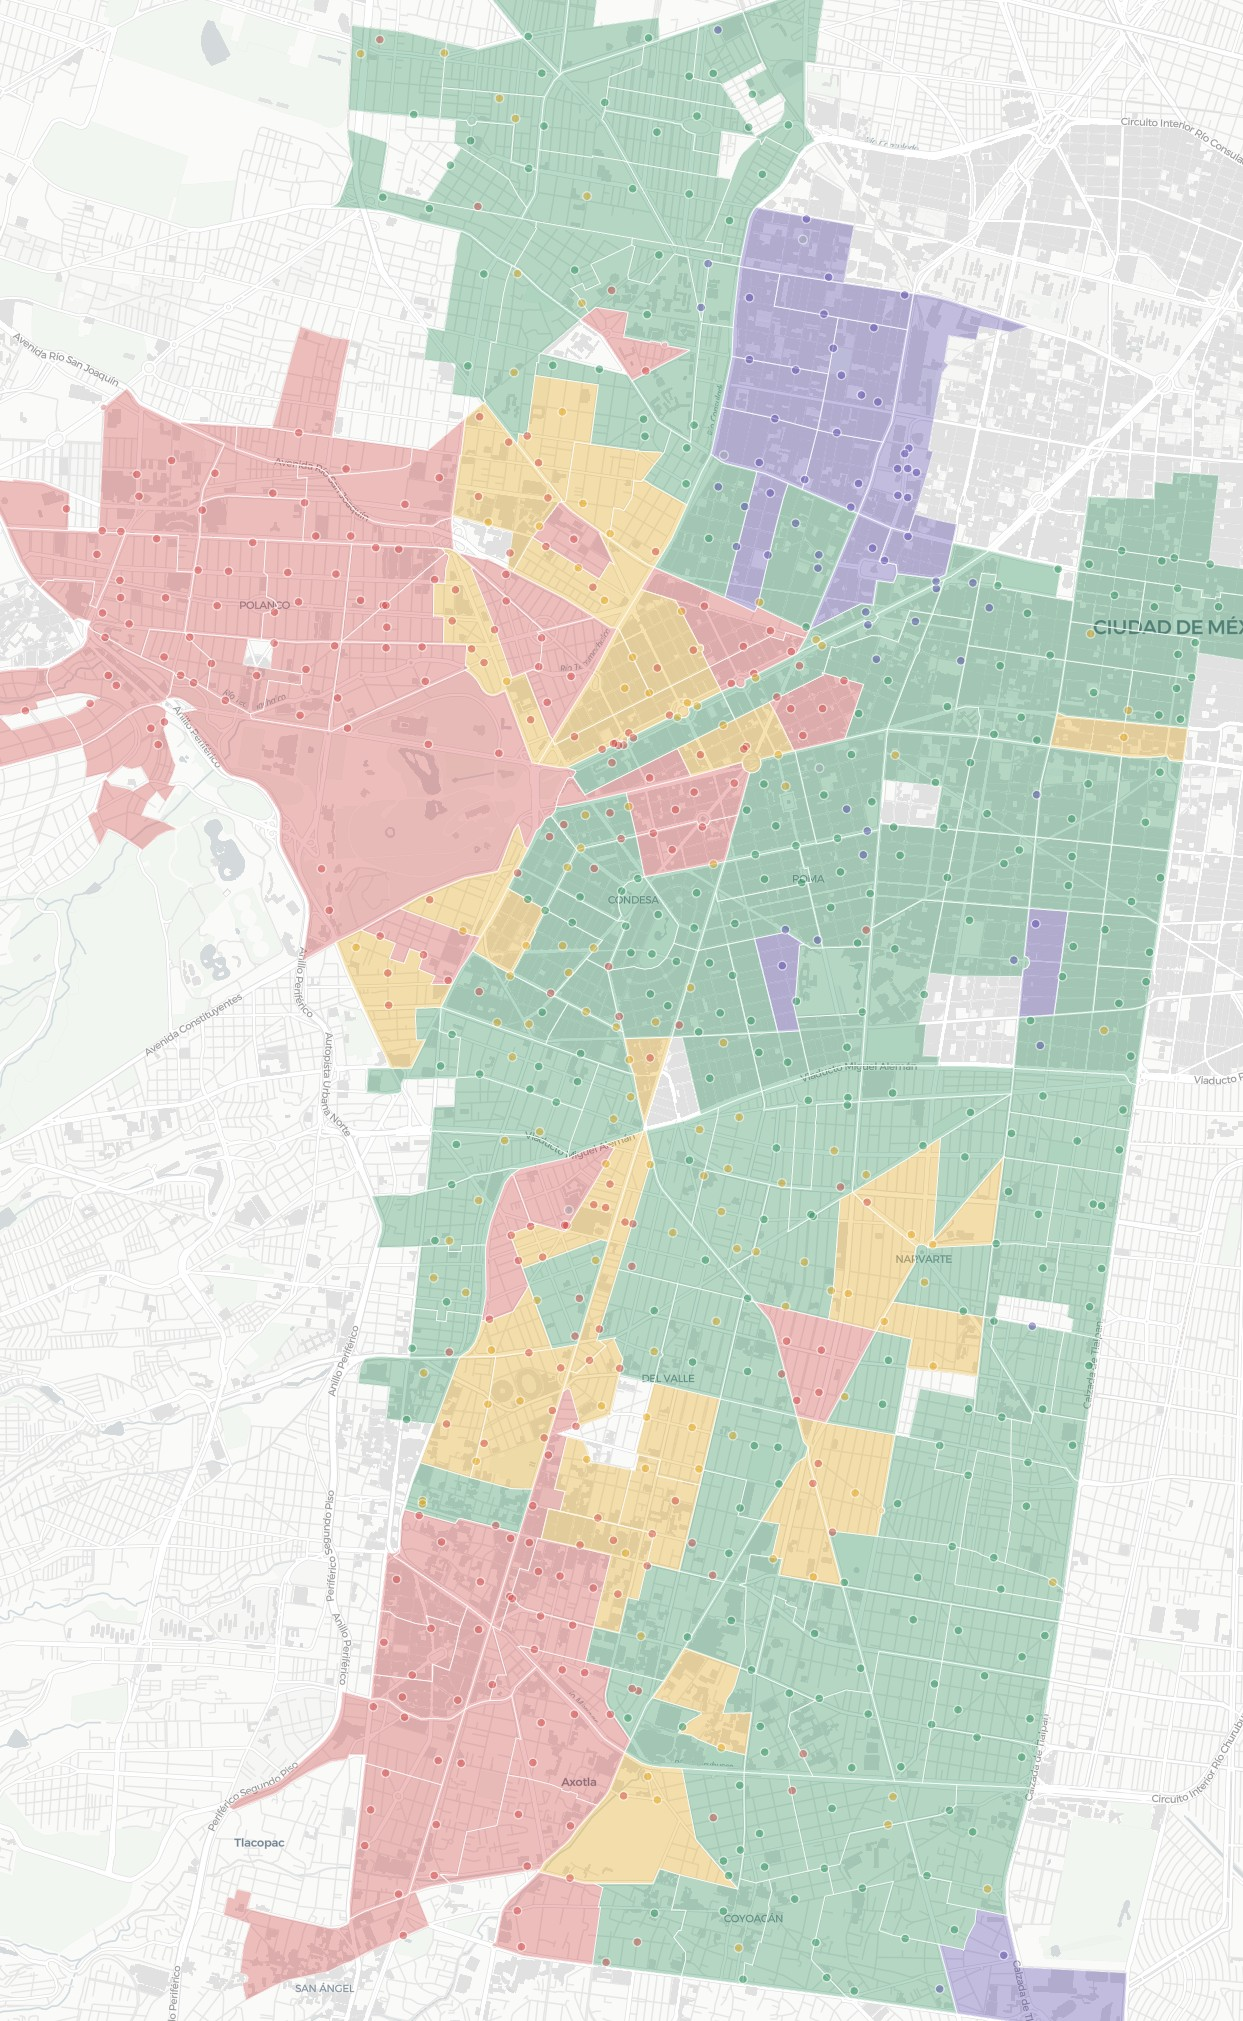
\includegraphics[height=2.1in]{figs/app-caso/sin-2100-col.jpg}
\caption{Sin rebalanceo, a las 9:00 (izquierda) y a las 21:00 (derecha). Cada AGEB del INEGI \cite{inegi_mg2024} suma las bicis disponibles y los anclajes libres de sus estaciones: rojo, sin bicis; amarillo, de 1 a 3; verde, más de 3; morado, sin anclajes libres.}
\label{fig:sin}
\end{figure}

Conviene aclarar de dónde sale esta figura. La produce nuestro simulador, que repite los viajes reales de ese día sin que nadie mueva una sola bici. Ecobici ya rebalancea, así que no es lo que se vio en la calle, sino lo que se habría visto sin el trabajo de sus equipos.

\subsection{Cómo medimos el problema}\label{sec:metricas}
Medimos el problema en minutos-estación. Llamamos $E$ a los minutos-estación con cero bicis disponibles y $F$ a los minutos-estación con cero anclajes libres; un minuto-estación es una estación durante un minuto, de modo que diez estaciones vacías durante una hora suman 600. $\EF$ mide cuánto tiempo el sistema no sirve a quien llega a sacar o a dejar una bici. Como segunda métrica contamos los desvíos, es decir, los viajes que no pueden salir de su estación porque está vacía, o terminar en ella porque está llena, y que el simulador manda a la estación más cercana que sí puede atenderlos; los reportamos por cada 100 salidas. Las dos métricas no miden lo mismo, porque $\EF$ pesa igual un minuto vacío en cualquier estación, mientras que los desvíos se acumulan donde hay más viajes.

Sumamos $E$ y $F$ con el mismo peso porque no encontrar bici y no poder dejarla son, para el usuario, el mismo problema: el sistema no le sirve. Se podría argumentar que quedarse sin bici es más grave, ya que impide empezar el viaje y es la queja más frecuente en la encuesta, pero preferimos no inventar una ponderación que no podemos medir y tratamos ambos minutos como equivalentes.

Con estas métricas se ve la importancia del rebalanceo (Tabla~\ref{tab:diferencia}). En promedio, sin rebalanceo el sistema acumularía \rbaseEF{} minutos-estación vacíos o llenos por día, y con el rebalanceo que medimos de Ecobici, \recoEF. El rebalanceo actual reduce el problema a menos de la mitad, y cualquier mejora sobre él depende de anticipar bien qué estaciones se van a vaciar o llenar.

\begin{table}[H]
\centering\footnotesize
\setlength{\tabcolsep}{4pt}
\caption{Lo que evita el rebalanceo de Ecobici, con los mismos viajes: sin rebalanceo y con los movimientos medidos de Ecobici. $E$, $F$ y $\EF$ en minutos-estación; desvíos por día; distancia media de un desvío en línea recta.}
\label{tab:diferencia}
\begin{tabular}{@{}lrrrr@{}}
\toprule
 & \multicolumn{2}{c}{1 sep. 2025} & \multicolumn{2}{c}{Media de \rdias{} días} \\
 & Sin rebal. & Ecobici & Sin rebal. & Ecobici \\
\midrule
$E$ & \cdBaseE & \cdEcoE & \rbaseE & \recoE \\
$F$ & \cdBaseF & \cdEcoF & \rbaseF & \recoF \\
$\EF$ & \cdBaseEF & \cdEcoEF & \rbaseEF & \recoEF \\
Desvíos & \cdBaseDesv & \cdEcoDesv & \cmBaseDesv & \cmEcoDesv \\
Distancia, m & \cdBaseKm & \cdEcoKm & \cmBaseKm & \cmEcoKm \\
\bottomrule
\end{tabular}
\end{table}

\subsection{Pregunta, hipótesis y alcance}
Considerando que trabajamos en un ambiente de información asimétrica, en el que no sabemos exactamente cómo rebalancea Ecobici, cuántas camionetas tiene ni a qué hora salen, nos preguntamos si es posible reconstruir su logística a partir de los patrones de sus datos públicos y, con esa misma logística, construir modelos de pronóstico y algoritmos de asignación que mejoren el sistema. Nuestra hipótesis es que asignar bicis cada quince minutos a partir de un pronóstico de viajes reduce $\EF$ frente al rebalanceo actual de Ecobici con el mismo esfuerzo.

El trabajo se centra en saber si el pronóstico mejora o no el rebalanceo. Decidimos cuántas bicis recoger o entregar en cada estación, con topes de esfuerzo y tiempos de traslado tomados de la operación de Ecobici, pero no trazamos las rutas de las camionetas ni calculamos cuántos vehículos harían falta. Todo el análisis ocurre dentro de un simulador, por lo que el resultado es una comparación entre políticas y no una medición en la calle.

% ======================================================================
\section{Supuestos}\label{sec:supuestos}
\subsection{Planteamiento}
Dividimos el trabajo en tres partes. La primera consiste en reconstruir lo que hace Ecobici a partir de sus datos públicos. La segunda es la asignación, en la que suponemos conocidos los viajes que saldrán y llegarán a cada estación y buscamos la mejor manera de repartir las bicis. La resolvemos con un procedimiento greedy que arma la decisión por paquetes, cada uno con una estación que recibe y las estaciones que le dan las bicis (Sección~\ref{sec:asignador}), porque hay que repartir un cupo común de visitas entre cientos de estaciones y garantizar que lo que se recoge sea igual a lo que se entrega, dos condiciones que una regla de umbrales por estación no puede imponer. En las tres partes, un minuto vacío y uno lleno pesan lo mismo (Sección~\ref{sec:metricas}). La tercera parte es construir un pronóstico que se acerque lo más posible a ese conocimiento perfecto. Dado lo ruidosa que es la demanda de cada estación, una media móvil es una referencia difícil de superar; aun así probamos LightGBM \cite{ke2017lightgbm}, que capta interacciones entre estación, hora y día sin especificarlas a mano.

\subsection{Datos}\label{sec:fuentes}
Trabajamos con cuatro fuentes públicas. La primera es el estado en vivo de las estaciones, un conjunto de archivos JSON en el estándar GBFS \cite{gbfs} que Ecobici actualiza cada diez segundos con las bicis disponibles, las no rentables y los anclajes libres de cada estación. Ese feed, sin embargo, es efímero: muestra solo el presente y no queda guardado en ningún lado, al menos no para el público. La segunda fuente resuelve ese problema. Max Halford mantiene un repositorio de código abierto, \texttt{bike-sharing-history} \cite{halford_bsh}, que consulta el feed cada unos quince minutos y archiva cada foto, de modo que contamos con un histórico por estación. Como esas fotos no bastan para saber qué pasó entre una y otra, las cruzamos con la tercera fuente, los viajes que Ecobici publica cada mes en datos abiertos \cite{ecobici_datos}, con la bici, las estaciones y la hora exacta de cada viaje (los campos están en el Apéndice~\ref{ap:campos}). La cuarta fuente son las AGEB urbanas del INEGI \cite{inegi_mg2024}, que usamos solo para visualizar.

Este cruce es relevante porque estamos en un ambiente de información asimétrica: no conocemos los rebalanceos exactos de Ecobici, ni cuántas camionetas tiene o a qué hora salen, así que todos esos números los inferimos de los datos con los supuestos que siguen. Suponemos que no hay datos no observados más allá de los huecos del histórico de fotos, que aparecen cuando el repositorio tarda más de quince minutos entre una consulta y la siguiente; la mediana entre fotos es de \rhuecoMed{} minutos, pero entre las 18:00 y las 21:59 sube a \rhuecoTarde. No inventamos fotos para cubrir esos huecos. Cuando falta una, el intervalo simplemente es más largo, observamos solo el cambio neto entre las dos fotos que sí existen y la estación conserva el valor de la última foto hasta que llega la siguiente. A veces una estación reporta una foto en blanco, con todos sus campos en cero; esas fotos las ignoramos al medir movimientos, porque no dicen nada sobre la estación. Además, solo usamos los días en los que al menos el \rcovMin\% de las horas tiene alguna foto, para que los huecos no dominen la medición. En 2025 cumplen \cvOkVeinticinco{} de \cvDiasVeinticinco{} días; en la prueba se descarta el \cvDiaExcl{} (\cvOkPrueba{} de \cvDiasPrueba), y el entrenamiento de los pronósticos no se afecta, porque usa los viajes del CSV (Apéndice~\ref{ap:cobertura}). El archivo guarda cada foto unos \rlagS{}~s después del estado que describe, así que restamos ese desfase antes de cruzarla con los viajes; las dos fuentes se unen por número de estación y por hora.

\subsection{Rebalanceo de Ecobici}\label{sec:medicion}
Hay dos maneras de saber si Ecobici rebalanceó. La primera sigue a cada bici por su identificador y detecta cuándo salta de la estación donde terminó un viaje a otra donde empieza el siguiente. Es un método frágil, porque si una bici desaparece varios días no sabemos qué ocurrió en medio, y un salto no dice cuántas bicis se movieron juntas. La segunda, que es la que usamos, compara en cada estación el cambio de bicis entre dos fotos con lo que explican los viajes. Entre dos fotos consecutivas $t_0$ y $t_1$ de la estación $i$,
\begin{equation}\label{eq:delta}
\delta_i=\Delta b_i+\Delta d_i-(a_i-s_i),
\end{equation}
donde $b$ son las bicis disponibles, $d$ las no rentables, y $a$ y $s$ las llegadas y salidas con hora en $(t_0,t_1]$. Lo que el cambio de bicis no explica con viajes lo atribuimos a Ecobici, y cada $\delta_i\neq0$ cuenta como una visita. El método da un piso del esfuerzo real, porque si en un intervalo traen una bici y se llevan tres solo vemos $-2$.

Ecobici rebalancea siguiendo a la demanda con un pequeño retraso, en una ola de mañana y otra de tarde (Apéndice~\ref{ap:ecobici}).

\subsubsection{Cuántas visitas por cada 15 minutos}
En promedio, Ecobici hace \recoVis{} visitas y mueve \recoBicis{} bicis por día entre las 05:00 y las 00:30, unas \chVisQuince{} visitas y \chPorQuince{} bicis por cuarto de hora. Para fijar un tope de esfuerzo llevamos las visitas de cada intervalo entre fotos a una base de quince minutos (visitas $\times$ 15 / duración del intervalo), en todas las fotos de los \ctopeDias{} días válidos de \ctopePeriodo, incluidas las que no tienen ninguna visita, y tomamos como tope el percentil 95, \ctopeVis{} visitas por decisión; el \cfigVisBajoTope\% de las fotos queda en el tope o por debajo (Fig.~\ref{fig:topes}a).


\begin{figure}[!htb]
\centering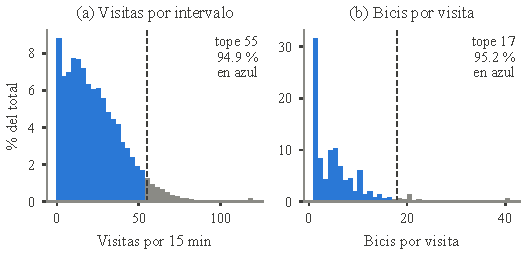
\includegraphics[width=\columnwidth]{figs/caso-topes.pdf}
\caption{Esfuerzo de Ecobici en los \ctopeDias{} días válidos de \ctopePeriodo, sin pares; es la misma población de la que salen los topes. (a) Visitas por intervalo entre fotos, llevadas a 15 minutos (\cfigIntervalos{} intervalos, incluido el \cfigSinVisita\% sin visitas; 120 incluye valores mayores). (b) Bicis por visita (\cfigVisitas{} visitas; 40 incluye valores mayores). En azul, lo que queda hasta el tope.}
\label{fig:topes}
\end{figure}

\subsubsection{Cuántas bicis por visita}
La mitad de las visitas mueve \cfigMedBicis{} bicis o menos, y el \cfigUnaDos\% solo una o dos. El percentil 95 es de \ctopeBicis{} bicis, que usamos como tope por visita; el \cfigBajoTope\% de las \cfigVisitas{} visitas queda en el tope o por debajo (Fig.~\ref{fig:topes}b). Ninguno de los dos porcentajes es exactamente 95: el percentil de visitas es \cfigVisPNoventaCinco{} y lo redondeamos a \ctopeVis, y las bicis por visita son enteras, así que todas las visitas de exactamente \ctopeBicis{} bicis quedan dentro.


Usamos el percentil 95 en los dos topes porque describe lo que Ecobici hace en un intervalo cargado sin tomar los extremos, que en parte son netos acumulados durante huecos largos entre fotos y no una sola parada de camioneta. Ambos topes salen de los \ctopeDias{} días válidos de \ctopePeriodo, entre las 05:00 y las 00:30. Son topes de esfuerzo y no describen una flota.

\subsubsection{Bodega y bicis no rentables}
En el largo plazo, el flujo neto de bicis entre la bodega y las estaciones es nulo: de un día al siguiente la flota anclada a las 04:45 cambia en promedio \cbMedia{} bicis (IC95 de \cbLo{} a $+$\cbHi). Por eso nuestro modelo no puede meter ni sacar bicis de bodega: solo las mueve entre estaciones, y cada decisión entrega exactamente lo que recoge. Las bicis no rentables cuentan en la ecuación~\eqref{eq:delta} para que un cambio de etiqueta no parezca una visita, y el simulador aplica cada cambio de etiqueta observado igual para todas las políticas; el detalle de ambos supuestos está en el Apéndice~\ref{ap:ecobici}.

\subsection{Logística de entrega}
Suponemos que una orden emitida en el minuto $t$ recoge sus bicis en $t+\rpickMin$ y las entrega en $t+\rdelMin$, es decir, quince minutos para llegar a la estación de origen y cargar, y cuarenta y cinco para el traslado y la descarga. Una hora nos parece suficiente, sobre todo si las camionetas están repartidas en distintas zonas de la ciudad, como las microzonas con que opera Ecobici \cite{mbn2026}. Al consultar aplicaciones de tráfico como Waze, los trayectos más largos entre estaciones llegan a unos 70 minutos en hora pico. Consideramos que no hay muchas horas pico en el día y que solo los trayectos más largos pasan de una hora, así que el supuesto nos parece sensato. La ruta por calle entre pares de estaciones al azar lo confirma: la mediana es de \rcalleMed{}~km y, a la velocidad media en hora pico de 13.5 km/h que reporta TomTom \cite{tomtom2025}, el par mediano toma \rpicoMed{} minutos, el percentil 90 \rpicoNoventa{} y el 99 \rpicoNN. Aun así, algunos traslados que propone el asignador unen estaciones lejanas. El supuesto de una hora sigue siendo aceptable, pero para reforzar su validez el asignador también puede preferir donantes cercanos con un costo por kilómetro, $\alpha$ (Secciones~\ref{sec:asignador} y~\ref{sec:alfa}). Es, además, el supuesto que más pesa: si la entrega ocurre a los \rentregaLarga{} minutos, el $\EF$ de la media móvil sube \rsSetenta{} minutos-estación por día (Sección~\ref{sec:sens}).

\subsection{Viajes y desvíos}
El simulador repite cada viaje del registro a su segundo exacto y ninguno se cancela. Por la forma en que lo simulamos, un viaje que no puede salir de su estación porque está vacía sale de la estación más cercana que tenga una bici en ese momento, y uno que no puede terminar en la suya porque está llena termina en la más cercana con un anclaje libre. Es lo más cercano que tenemos para mantener la demanda fija entre políticas: en la realidad parte de esas personas desistiría, y como los registros solo contienen los viajes que sí ocurrieron, la demanda real está censurada \cite{negahban2019}. Por eso tratamos $E$, $F$ y los desvíos como exposición a la falla y no los traducimos a viajes perdidos o ganados. Además, en nuestra simulación hay desvíos falsos. Con los movimientos medidos de Ecobici, los viajes son literalmente los que sí ocurrieron y en la realidad ninguno se desvió, pero el simulador desvía varios, sobre todo por los desfases del feed que describimos a continuación (Sección~\ref{sec:fidelidad}).

\subsection{Desfases entre el feed y los viajes}
El feed y los viajes no están sincronizados al segundo. Si una bici sale unos segundos antes de una foto, la foto todavía la muestra anclada; la ecuación~\eqref{eq:delta} da $+1$ en ese intervalo y $-1$ en el siguiente, y aparece un par que se deshace (un ejemplo real está en el Apéndice~\ref{ap:auditoria}). Por eso un movimiento que se deshace exactamente en el intervalo siguiente, en la misma estación, no cuenta como visita. Sin esta regla Ecobici tendría \rvisSinRegla{} visitas por día y con ella \rvisConRegla, el \rvisQuedan\%; la regla reduce el esfuerzo que le medimos, lo que nos pone una vara más alta, y la aplicamos igual a nuestras órdenes (Apéndice~\ref{ap:auditoria}). El mismo desfase hace que nuestra simulación de Ecobici no coincida exactamente con la realidad, como veremos en la Sección~\ref{sec:fidelidad}. Por último, Ecobici presta bicis de 05:00 a 00:30 \cite{ecobici_horario}, y esa es la ventana que simulamos.

% ======================================================================
\section{Resultados y discusión}\label{sec:resultados}
\subsection{El simulador}
El simulador es sencillo. Cada día arranca a las 05:00 sin viajes en curso, con el estado de cada estación según la primera foto del día, y a partir de ahí ya no vuelve a mirar las fotos: solo reproduce los viajes registrados, cada uno a su segundo exacto. Lo hacemos así porque las fotos ya incorporan el rebalanceo de Ecobici; si el simulador siguiera el estado observado de las estaciones durante el día, ese rebalanceo quedaría mezclado con el de la política evaluada y no sería posible aislar el efecto de esta última. Sobre los viajes aplicamos las recogidas y entregas de la política que se prueba y los cambios de no rentable a rentable observados, que son los mismos para todas. Lo único que puede cambiar entre una política y otra es que un viaje no pueda salir porque su estación está vacía, o no pueda terminar porque está llena; en ese caso lo mandamos a la estación más cercana que sí pueda atenderlo y lo contamos como desvío. Cada minuto contamos qué estaciones están vacías y cuáles llenas para obtener $E$ y $F$.

Una orden emitida a las 08:00 recoge a las 08:15 y entrega a las 09:00, y el simulador no la aplica a ciegas, porque en ese tiempo los viajes cambiaron el inventario de las estaciones. Cada paquete del asignador (Sección~\ref{sec:asignador}) viaja por separado: las bicis que recogen sus donantes solo van a su receptor. Al llegar a recoger, la camioneta se lleva lo pedido, hasta \ctopeBicis{} bicis por visita; si en la estación ya no hay tantas, se lleva solo las que haya y no completa en otra estación, así que el receptor recibe solo lo que se alcanzó a cargar. Al llegar a entregar, deja las bicis en el destino; las que no caben, o todas si el destino está fuera de servicio, las deja en la estación con anclajes libres más cercana a ese destino. Las bicis nunca vuelven a su estación de origen. Ninguna bici se crea ni se pierde, y una verificación lo comprueba después de cada evento. Esto ocurre poco: con la media móvil, de \coRecogidas{} bicis recogidas por día, faltaron \coFalta{} al llegar a recoger (el \coFaltaPct\% de lo pedido) y \coDevueltas{} no cupieron en su destino (el \coDevueltasPct\%). Para el brazo de Ecobici no hay órdenes: aplicamos sus movimientos medidos $\delta_i$ a la hora de la segunda foto de cada intervalo.

\subsection{El asignador greedy}\label{sec:asignador}
Cada quince minutos, en el minuto $t$, el asignador decide de qué estaciones sacar bicis y a cuáles llevarlas para que en las próximas $n$ horas haya menos minutos con estaciones vacías o llenas. La idea es sencilla. Primero proyecta cuántas bicis tendrá cada estación si nadie interviene. Después prueba, estación por estación, qué pasaría si le quitara o le metiera bicis, y cuánto ganaría o perdería en minutos vacíos o llenos. Con eso ordena a las estaciones que más necesitan bicis, los receptores, y a cada una, empezando por la que más lo necesita, le arma un paquete con las estaciones que mejor pueden darle bicis, sus donantes. Sigue así, un paquete a la vez, hasta que llega al límite de visitas o hasta que el siguiente paquete ya no vale la pena. A esta forma de decidir, que en cada paso toma lo que más conviene en ese momento y no vuelve atrás, se le llama greedy. Lo que decide se vuelve órdenes que se recogen en $t+\rpickMin$ y se entregan en $t+\rdelMin$; no se cancelan, y en la decisión siguiente cuentan como órdenes pendientes.

El primer paso es la proyección. De cada estación $i$ conocemos las bicis disponibles que tiene en $t$, $b_i$, y cuántas caben en total, $K_i$, que es la suma de las disponibles y los anclajes libres. Está vacía cuando su inventario es 0 y llena cuando es $K_i$. El pronóstico dice cuántos viajes llegarán y saldrán cada hora; lo repartimos en partes iguales entre los cuatro cuartos de hora y lo convertimos en un flujo neto por minuto, $f_{im}=(\text{llegadas}-\text{salidas})/60$, que es positivo si la estación recibe más bicis de las que pierde y negativo si pasa lo contrario. Con eso, la ecuación siguiente calcula cuántas bicis tendrá la estación en cada minuto futuro si nadie más interviene, salvo por las órdenes que ya están en camino: parte de $b_i$ y avanza un minuto a la vez.
\begin{equation}\label{eq:proy}
s_i(m+1)=\bigl[\,[\,s_i(m)+o_{im}\,]_{K_i}+f_{im}\bigr]_{K_i},\qquad s_i(0)=b_i.
\end{equation}
En cada minuto se aplica primero lo que traen las órdenes pendientes, $o_{im}$ (las bicis que una orden ya emitida entrega, con signo positivo, o recoge, con signo negativo, en esa estación en el minuto $m$), y después el flujo $f_{im}$. El corchete $[a]_K=\min\{K,\max\{0,a\}\}$ recorta el resultado entre 0 y $K_i$, porque una estación no puede tener menos de cero bicis ni más de las que le caben. De esta proyección tomamos dos valores: $p_i$, el inventario esperado cuando la camioneta llegue a recoger ($m=\rpickMin$), y $q_i$, el esperado cuando llegue a entregar ($m=\rdelMin$). Con ellos sabemos cuánto puede dar o recibir cada estación en una visita: a lo más se recoge lo que habrá, $r_i=\min(B,\lfloor p_i\rfloor)$, y a lo más se entrega lo que cabrá, $u_i=\min(B,\lfloor K_i-q_i\rfloor)$, donde $B$ es el tope de bicis por visita y $\lfloor\cdot\rfloor$ redondea hacia abajo, porque no existen las medias bicis.

El segundo paso es medir cuánto gana o pierde cada estación con cada cantidad, y se hace con dos tablas para todas las estaciones. Antes de decidir no sabemos si a una estación le conviene dar o recibir bicis, y muchas podrían hacer cualquiera de las dos cosas, porque tienen bicis y también anclajes libres. Por eso a cada estación le preguntamos las dos cosas. La primera tabla responde: si a las $t+\rpickMin$ le quitamos una bici, ¿cuántos minutos más, o menos, pasaría vacía o llena? ¿Y si le quitamos dos, tres, y así hasta $B$? La segunda responde lo mismo al meterle de una hasta $B$ bicis a las $t+\rdelMin$. Cada respuesta sale de repetir la proyección~\eqref{eq:proy} con ese cambio y compararla con la proyección sin cambio, desde el momento de la visita hasta el final del horizonte, $H=\min\{60n,\ \text{minutos hasta las 00:30}\}$. De cada tabla solo cuentan las cantidades posibles: hasta $r_i$ bicis para quitar y hasta $u_i$ para meter. Para recoger $k$ bicis esto se representa con
\begin{equation}\label{eq:costo}
c^R_i(k)=\sum_{m=\rpickMin+1}^{H}\bigl(v_i(s^{-k}_i(m))-v_i(s_i(m))\bigr),
\end{equation}
donde $s^{-k}_i$ es la proyección con las $k$ bicis menos, $s_i$ la proyección sin cambio y $v_i(s)$ vale 1 si con $s$ bicis la estación cuenta como vacía o llena ($s<\tfrac12$ o $s>K_i-\tfrac12$) y 0 si no. Para entregar $x$ bicis, $c^E_i(x)$ es la misma suma con $x$ bicis más en el minuto $\rdelMin$, contada desde ahí. Las dos son el cambio total en minutos-estación por mover esas $k$ o $x$ bicis en una sola visita, no un costo por bici. Como se miden contra no hacer nada, sin mover bicis el cambio es cero y un valor negativo es un ahorro. Recoger suele costar minutos, porque la estación se vacía antes, y entregar suele ahorrarlos, salvo que la llene. El parámetro $n$ es cuántas horas hacia adelante mira el asignador: con $n=1$ no puede actuar, porque la entrega cae justo al final y no alcanza a cambiar nada, y con $n$ mayor ve más consecuencias pero se apoya en pronósticos más inciertos.

Mover bicis no es gratis, así que cada visita tiene un precio. Lo representamos con $\lambda$, en minutos-estación, que se cobra una vez por cada parada de la camioneta, sin importar cuántas bicis mueva: recoger una bici o dos en la misma estación paga un solo $\lambda$. Así, una visita solo conviene si lo que ahorra supera su $\lambda$, y con una $\lambda$ alta el asignador hace menos visitas y mueve más bicis en cada una.

La distancia tampoco es gratis. Para que el asignador prefiera donantes cercanos le agregamos un segundo precio, $\alpha$, en minutos-estación por kilómetro: cada tramo de un donante $j$ a su receptor $i$ cuesta además $\alpha D_{ij}$, donde $D_{ij}$ son los kilómetros en línea recta entre las dos estaciones. Con $\alpha=0$ la distancia no cuenta, que es el caso de los resultados principales; con $\alpha$ mayor el asignador cambia donantes lejanos por cercanos a cambio de un poco más de $\EF$ (Sección~\ref{sec:alfa}).

El tercer paso es armar los paquetes, y ahí cada tabla tiene un papel distinto. El procedimiento recorre los receptores y a cada uno le busca donantes; es una elección de cómo armar la decisión. Con la tabla de entregar, $c^E$, se ordenan los receptores según cuánto ganarían si las bicis les llegaran gratis, es decir, el mejor ahorro de su entrega menos el precio de su propia visita,
\begin{equation}\label{eq:g}
g_i=\max_{1\le x\le u_i}\bigl(-c^E_i(x)-\lambda\bigr).
\end{equation}
La tabla de recoger, $c^R$, es la contraparte: dice cuánto cuesta sacar las bicis que ese receptor necesita. Con ella los donantes de cada receptor $i$ se ordenan del más barato al más caro, según lo que cuesta cada bici que dan cuando se reparte el precio de la visita y del tramo entre todas las bicis que se llevan,
\begin{equation}\label{eq:rho}
\rho_{ij}=\min_{1\le k\le r_j}\frac{c^R_j(k)+\lambda+\alpha D_{ij}}{k};
\end{equation}
así, un donante que puede dar muchas bicis sin vaciarse, y que está cerca, va primero. Con esos dos órdenes, el asignador toma al receptor con mayor $g_i$ y prueba entregarle una bici, dos, y así hasta $u_i$. Para cada cantidad $x$ junta las bicis de los donantes todavía libres, del más barato al más caro, tomando de cada uno lo que le falta para completar $x$ o todo lo que puede dar, $k_j=\min(\text{falta},\,r_j)$. El paquete junta las dos tablas: su costo neto es lo que dice $c^E$ de la entrega más su visita, y lo que dice $c^R$ de cada recogida más su visita y su tramo,
\begin{equation}\label{eq:paquete}
C_i(x)=c^E_i(x)+\lambda+\textstyle\sum_{j}\bigl(c^R_j(k_j)+\lambda+\alpha D_{ij}\bigr),
\end{equation}
y de todas las cantidades se queda con la de mayor ahorro neto, $-C_i(x)$. Si ese ahorro es positivo, el paquete se acepta: el receptor recibe $x$ bicis y cada donante entrega sus $k_j$. Esas estaciones quedan usadas y ya no entran en otro paquete de la misma decisión, ni para dar ni para recibir, así que aunque una estación tenga abiertas las dos opciones, en una decisión solo hace una. Luego pasa al siguiente receptor de la lista y repite.

Cada paquete recoge exactamente lo que entrega, porque sus $k_j$ suman $x$. Como la decisión es la suma de sus paquetes, también recoge lo mismo que entrega, y la bodega no gana ni pierde bicis.

El procedimiento se detiene por dos razones distintas. La primera es un límite duro de esfuerzo, tomado de lo que hace Ecobici: el percentil 95 de todo 2025 (Sección~\ref{sec:medicion}), que da $V=\ctopeVis$ visitas por decisión y $B=\ctopeBicis$ bicis por visita. El tope de bicis se aplica desde el principio, porque $r_i$ y $u_i$ nunca pasan de $B$. El de visitas se aplica mientras se arman los paquetes: un paquete con $d$ donantes usa $1+d$ visitas y solo se acepta si cabe en las que quedan, y cuando ya no caben dos visitas, el mínimo de un paquete, el procedimiento termina. No se recorta al final porque quitar visitas de una decisión ya armada rompería paquetes: un receptor sin uno de sus donantes recibiría menos bicis de las que se evaluaron. La segunda razón es que el procedimiento también para antes por sí solo, aunque todavía quepan visitas, cuando lo que sigue no vale la pena. Si el siguiente receptor tiene $g_i\le0$, ni con bicis gratis su entrega pagaría su visita, y como los receptores van ordenados, los que siguen tampoco; ahí termina la decisión. Si un receptor sí ahorra pero el paquete con sus donantes cuesta más de lo que ahorra, ese paquete no se hace y se pasa al siguiente. Cuando ya no quedan donantes libres, ningún paquete nuevo se completa. Por eso hay decisiones que usan muchas menos visitas que el tope.

Lo que sale de cada decisión es una orden por estación visitada, recoger $k_j$ o entregar $x$, con el número de su paquete, de modo que se sabe de dónde a dónde va cada bici. Todas se recogen en $t+\rpickMin$ y se entregan en $t+\rdelMin$. Quince minutos después se repite todo con el estado nuevo, y las órdenes emitidas que aún no se ejecutan entran a la proyección como $o_{im}$.

El procedimiento tiene límites. No garantiza la mejor decisión posible, solo una buena y rápida. Un donante sirve a un solo receptor por decisión, aunque le sobren bicis después de completar su paquete. Y la distancia solo entra por $\alpha$ y en línea recta, no por calle, mientras que todas las órdenes usan la misma hora de traslado.

\subsection{Los pronósticos}
Los pronósticos estiman cuántos viajes saldrán y llegarán a cada estación en cada hora. La forma diaria se calcula una sola vez a las 05:00 para todo el día; la directa se recalcula en cada decisión para las horas siguientes, usando lo que ya pasó ese día. La media móvil, en forma diaria, promedia para cada estación y hora los conteos de los días del mismo tipo (entre semana, o fin de semana y festivo) de las \rsemanasHist{} semanas previas, sin entrenar nada.

LightGBM diario usa dos modelos de árboles con potenciación de gradiente, uno para salidas y otro para llegadas, con pérdida Poisson porque el objetivo es un conteo. Cada fila es una estación en una hora del día, descrita por la estación, la hora, el día de la semana, si es festivo, los conteos de esa hora hace 7 y 14 días y la media móvil. Sus parámetros son fijos y no se buscaron (\rlgbArboles{} árboles, tasa de \rlgbTasa, \rlgbHojas{} hojas). LightGBM directo agrega cuántas horas adelante se pronostica, los viajes de la estación en el último cuarto de hora y en la última hora, y cuánto va el día por encima o por debajo de un día típico a esa misma hora; todo con información anterior a la decisión.

Para saber qué tan bien pronostica cada uno, medimos cada pronóstico contra los viajes reales de los \cfMeses{} meses de prueba, por estación y por hora. El MAE es el error absoluto medio, en viajes; el WAPE es el error absoluto total entre el total de viajes reales, de modo que un 40\% significa que el pronóstico se equivoca, en conjunto, por una cantidad igual al 40\% de los viajes. La Tabla~\ref{tab:pron} del Apéndice~\ref{ap:ecobici} los da para salidas, llegadas y su neto (lo que usa el asignador), en la primera hora y en la cuarta, la última que mira; la media móvil se equivoca en \cfMaeMaPri{} viajes por estación y hora en el neto y por el \cfWapeMaSal\% del total en las salidas. LightGBM diario es apenas mejor (\cfDifDPri\% menos error en el neto de la primera hora, \cfDifDUlt\% en la cuarta); LightGBM directo, que además usa lo ocurrido ese día, es peor (\cfDifDirPri\% y \cfDifDirUlt\% más error). Como un error chico en una estación crítica puede costar más $\EF$ que varios en una holgada, también los comparamos por el $\EF$ que logran con el asignador.


Los modelos nunca ven el futuro: cada mes se pronostica con modelos entrenados en meses anteriores (Sección~\ref{sec:calibracion} y Apéndice~\ref{ap:ventanas}). Construimos además dos oráculos que reciben los conteos reales de cada hora del día. No son una estrategia posible: marcan el techo de lo que lograría el mismo asignador con un pronóstico perfecto.

\subsection{Entrenamiento, validación y prueba}\label{sec:calibracion}
Separamos los días en tres bloques consecutivos, para que nada de lo que se evalúa haya servido para ajustar algo. El \emph{entrenamiento} son los viajes de enero a julio de 2025, con los que se entrenan los LightGBM que se usan en la validación. La \emph{validación} son todos los días de \rselMes{} con al menos el \rcovMin\% de sus horas cubiertas por fotos, \rselDias{} en total; ahí, y solo ahí, se eligen $n$ y $\lambda$, que después se congelan. La \emph{prueba} son todos los días válidos de \rpruebaPeriodo, \rdias{} en total, y es móvil: cada mes los LightGBM se vuelven a entrenar con los \rtrainMeses{} meses anteriores, de modo que el de septiembre ya incluye agosto como historia, y la media móvil solo usa las \rsemanasHist{} semanas previas a cada día (Fig.~\ref{fig:ventanas}). En la prueba no se ajustó nada. No usamos 2026: el archivo de fotos de ese año es más sucio, y preferimos la comparación más justa contra Ecobici.

Elegimos $n$ con los dos oráculos: el primer horizonte cuyo siguiente ya no mejora $\EF$ de forma demostrable, $n=\rnDiario$ para la forma diaria y $n=\rnDirecto$ para la directa. Para comparar con el mismo esfuerzo, a cada brazo le buscamos la $\lambda$ con la que hace tantas visitas por día como Ecobici en la validación, \rselEcoVis; quedaron \rlamMa{} para la media móvil, \rlamLgbmD{} y \rlamLgbmDir{} para los dos LightGBM, y \rlamOrD{} y \rlamOrDir{} para los oráculos (el procedimiento de ambos está en el Apéndice~\ref{ap:ventanas}). Con esas $\lambda$, el mejor pronóstico real en la validación fue la \rmejorReal.

\subsection{Resultados}
La Tabla~\ref{tab:principal} resume los siete brazos. Sin rebalanceo, el sistema acumula \rbaseEF{} minutos-estación vacíos o llenos por día y el rebalanceo medido de Ecobici lo baja a \recoEF. La media móvil con el asignador llega a \rmaEF, \rmaPct\% menos que Ecobici (IC95 de \rmaPctLo{} a \rmaPctHi\%), con menos tiempo vacío (\rmaE{} contra \recoE) y mucho menos tiempo lleno (\rmaF{} contra \recoF). Gana en los \rmaGana{} días con \rmaVis{} visitas y \rmaBicis{} bicis movidas por día, frente a \recoVis{} y \recoBicis{} de Ecobici, y la mejora se mantiene en \rdicMes, el último mes de prueba (\rdicPct\%). Nuestra hipótesis se cumple.

\begin{table*}[!htb]
\centering\footnotesize
\caption{Medias por día en \rdias{} días de prueba, con $n=\rnDiario$ horas en los cinco brazos con asignador. $E$, $F$ y $\EF$ en minutos-estación; Desv.: viajes desviados por cada 100 salidas; m/desv.: distancia media de un desvío. Última columna: reducción de $\EF$ frente a Ecobici, con IC95, en porcentaje del $\EF$ medio de Ecobici.}
\label{tab:principal}
\begin{tabular}{@{}lrrrrrrrl@{}}
\toprule
Brazo & E & F & E+F & Visitas & Bicis & Desv., \% & m/desv. & Menos E+F, \% [IC95] \\
\midrule
Sin rebalanceo & 169,276 & 50,785 & 220,061 & 0 & 0 & 27.0 & 383 & --- \\
Ecobici (medido) & 84,956 & 17,178 & 102,135 & 2,263 & 10,276 & 4.4 & 259 & --- \\
Media móvil & 53,774 & 4,028 & 57,802 & 2,060 & 10,084 & 7.1 & 246 & 43.4 [41.2, 45.6] \\
LightGBM diario & 54,120 & 4,067 & 58,187 & 2,054 & 9,746 & 7.1 & 246 & 43.0 [40.9, 45.2] \\
LightGBM directo & 53,647 & 3,863 & 57,510 & 2,094 & 10,878 & 7.5 & 248 & 43.7 [41.6, 45.7] \\
\midrule
Oráculo diario & 38,078 & 2,794 & 40,872 & 2,054 & 9,908 & 5.0 & 248 & 60.0 [57.5, 62.5] \\
Oráculo directo & 30,934 & 2,751 & 33,684 & 2,054 & 8,851 & 3.6 & 236 & 67.0 [64.0, 70.1] \\
\bottomrule
\end{tabular}

\end{table*}

\begin{table*}[!htb]
\centering\footnotesize
\setlength{\tabcolsep}{3.2pt}
\caption{Costo por kilómetro ($\alpha$, minutos-estación por km) en los \caDias{} días de prueba, con la media móvil y la misma $n$ y $\lambda$. Medias por día; $\EF$ en minutos-estación; km de tramos: suma, en línea recta, de cada tramo donante $\to$ receptor; desvíos: viajes desviados por día. Columnas vs.: cambio en porcentaje frente a $\alpha=0$ y frente a Ecobici. Los km de Ecobici son una cota inferior (ver texto).}
\label{tab:alfa}
\begin{tabular}{@{}lrrrrrrrrrrrr@{}}
\toprule
 & \multicolumn{3}{c}{$\EF$} & \multicolumn{3}{c}{Bicis movidas} & \multicolumn{3}{c}{Km de tramos} & \multicolumn{3}{c}{Desvíos} \\
\cmidrule(lr){2-4}\cmidrule(lr){5-7}\cmidrule(lr){8-10}\cmidrule(l){11-13}
 & Por día & vs.\ $\alpha{=}0$ & vs.\ Eco. & Por día & vs.\ $\alpha{=}0$ & vs.\ Eco. & Por día & vs.\ $\alpha{=}0$ & vs.\ Eco. & Por día & vs.\ $\alpha{=}0$ & vs.\ Eco. \\
\midrule
Ecobici (medido) & 102,135 & --- & --- & 10,276 & --- & --- & $\ge$3,181 & --- & --- & 2,298 & --- & --- \\
\midrule
Media móvil, $\alpha=0$ & 57,802 & --- & $-$43.4 & 10,084 & --- & $-$1.9 & 4,927 & --- & $+$54.9 & 3,706 & --- & $+$61.3 \\
Media móvil, $\alpha=1$ & 58,161 & $+$0.6 & $-$43.1 & 9,972 & $-$1.1 & $-$3.0 & 3,728 & $-$24.3 & $+$17.2 & 3,761 & $+$1.5 & $+$63.7 \\
Media móvil, $\alpha=3$ & 59,027 & $+$2.1 & $-$42.2 & 9,766 & $-$3.2 & $-$5.0 & 3,179 & $-$35.5 & $-$0.1 & 3,823 & $+$3.1 & $+$66.3 \\
Media móvil, $\alpha=5$ & 59,761 & $+$3.4 & $-$41.5 & 9,635 & $-$4.4 & $-$6.2 & 2,875 & $-$41.6 & $-$9.6 & 3,871 & $+$4.4 & $+$68.4 \\
Media móvil, $\alpha=10$ & 61,526 & $+$6.4 & $-$39.8 & 9,373 & $-$7.0 & $-$8.8 & 2,421 & $-$50.9 & $-$23.9 & 3,965 & $+$7.0 & $+$72.5 \\
\bottomrule
\end{tabular}

\end{table*}

Los intervalos de la última columna comparan cada brazo con Ecobici día por día: para cada uno de los \rdias{} días calculamos la diferencia de $\EF$, y el intervalo es la media de esas diferencias más o menos el cuantil 0.975 de una $t$ de Student con un grado de libertad menos que el número de días, por su error estándar. Pareamos por día porque ambos brazos ven los mismos viajes, y así la variación entre días no ensancha el intervalo.

Los tres pronósticos reales empatan en $\EF$: sus intervalos se traslapan, LightGBM diario y directo no superan de forma apreciable a la media móvil, y su exactitud tampoco es mejor de forma apreciable (Tabla~\ref{tab:pron}), así que la ventaja viene de asignar con un pronóstico razonable y no de un modelo más complejo. Con los viajes reales, el mismo asignador llega a \rorDEF{} con el oráculo diario y a \rorDirEF{} con el directo. La distancia de \rmaGap{} minutos-estación entre la media móvil y su oráculo es lo que cuesta no conocer el futuro, y la diferencia de \roracleDirectGap{} entre los dos oráculos indica que, con información perfecta, actualizar el pronóstico cada quince minutos sí vale la pena; LightGBM directo no aprovecha esa ventaja y queda a \rlgbmDirGap{} de su oráculo.

El promedio podría esconder que la política solo gana en las horas tranquilas, así que comparamos Ecobici con LightGBM directo el \rejDia{} en las dos horas pico. Entre las 8:45 y las 9:00 (Fig.~\ref{fig:nueve}, en el Apéndice~\ref{ap:mapas}), Ecobici deja \csEcoNueveEF{} minutos-estación vacíos o llenos y LightGBM directo \csLgbmNueveEF.

Entre las 20:45 y las 21:00 (Fig.~\ref{fig:veintiuno}, en el Apéndice~\ref{ap:mapas}) la diferencia es de \csEcoVeintiunoEF{} contra \csLgbmVeintiunoEF, y en el día completo de \cdEcoEF{} contra \cdLgbmEF{} (Tabla~\ref{tab:dia}, en el Apéndice~\ref{ap:mapas}). Los desvíos van en sentido contrario: en el cuarto de hora de las 9:00 son \csEcoNueveDesv{} con Ecobici y \csLgbmNueveDesv{} con LightGBM, y en el día \cdEcoDesv{} contra \cdLgbmDesv.


Las dos métricas no cuentan lo mismo. Con la media móvil hay \rmaDesvPct{} desvíos por cada 100 salidas, contra \recoDesvPct{} de Ecobici simulado, aunque el oráculo directo desvía menos (\rorDirDesvPct). Nuestra explicación es que la política baja $\EF$ llenando estaciones de poca demanda y se queda corta en las de mucha, donde el pronóstico falla más. En los \rcfDias{} días guardados minuto a minuto, el décimo de estaciones con más viajes (\rdTop{} de \rdEst, con el \rdTopViajes\% de las salidas y llegadas) baja $\EF$ solo \rdEFTopRed\% frente a Ecobici simulado, contra \rdEFRestoRed\% en el resto; ahí sus minutos vacíos incluso suben (\rdETopMa{} contra \rdETopEco) y ahí cae el \rdMaExtraTop\% de sus desvíos de más.

\subsection{Amenazas a la validez}\label{sec:amenazas}
\subsubsection{Fidelidad del simulador}\label{sec:fidelidad}
Para saber qué tan fiel es el simulador comparamos las fotos con lo que da al repetir los movimientos medidos de Ecobici en los mismos \rdias{} días. En $\EF$ casi coinciden: \rfdFeedEF{} minutos-estación en las fotos (\rfdFeedE{} vacíos y \rfdFeedF{} llenos) y \recoEF{} en el simulador (\recoE{} y \recoF). En los desvíos no: en la realidad no hubo ninguno, y el simulador desvía \rfdEcoDesv{} viajes por día, el \recoDesvPct\% de las salidas; esa diferencia es del simulador, no de Ecobici. En los \rcfDias{} días guardados minuto a minuto encontramos tres causas: la resolución de las fotos, salidas desde estaciones que el feed marca vacías y el arrastre del inventario simulado, que no se vuelve a igualar con el feed (Apéndice~\ref{ap:fidelidad}). Por eso leemos los desvíos como una comparación entre brazos con los mismos viajes y no como una predicción de lo que ocurriría en la calle.

\subsubsection{Supuestos favorables a Ecobici}
Varios supuestos juegan en contra de nuestras políticas. La $\lambda$ se fijó para igualar las visitas de Ecobici en \rselMes, y en la prueba la media móvil hizo \rmaVisPct\% menos, así que la comparación no es a igual esfuerzo exacto, pero el error favorece a Ecobici. El neto de sus movimientos, que al reproducirse suma \recoNeto{} bicis por día dentro de la ventana, no tiene que ser cero, mientras que nuestras políticas no reciben bicis de fuera. Lo que medimos de Ecobici es un piso de su esfuerzo, porque solo vemos netos entre fotos, y al quitar los pares que se deshacen le bajamos el esfuerzo medido, lo que nos pone una vara más alta. Además, nuestras políticas no pueden llevarse una bici dañada y devolverla reparada, como sí puede Ecobici. Los topes de esfuerzo se miden sobre todo 2025, que incluye los meses de prueba, porque describen la operación de Ecobici y no son un parámetro ajustado a favor de nuestras políticas.

\subsubsection{Sensibilidad a los supuestos}\label{sec:sens}
Repetimos la media móvil y el oráculo directo en los \cxDias{} días de prueba cambiando un supuesto a la vez, con la misma $\lambda$ (Tabla~\ref{tab:sens}, en el Apéndice~\ref{ap:sens}). El tiempo de entrega es el más sensible: a los \rentregaLarga{} minutos en lugar de \rdelMin, el $\EF$ de la media móvil cambia \rsSetenta{} minutos-estación por día, y a los \rentregaCorta, \rsCuarenta; aun en el caso lento queda \cxLargaPct\% por debajo del Ecobici de esos días, contra \cxMaPct\% en el caso base. Tomar las bicis no rentables del feed pesa mucho menos, y la regla de pares solo cambia el esfuerzo que le medimos a Ecobici, no su $\EF$ (Apéndice~\ref{ap:auditoria}). Queda sin probar la logística: los topes no modelan rutas.

\subsubsection{Costo por kilómetro}\label{sec:alfa}
Para medir cuánto cuesta acortar los traslados repetimos la media móvil en los \caDias{} días de prueba con $\alpha\in\{\caAlfas\}$ minutos-estación por kilómetro y la misma $n$ y $\lambda$ (Tabla~\ref{tab:alfa}). Los de Ecobici no se observan, porque solo vemos cuántas bicis sacó y metió en cada estación; como referencia damos una cota inferior: emparejamos sus recogidas con sus entregas de la misma foto o de la hora siguiente de la forma que sume menos kilómetros, lo que cubre el \caEcoEmpar\% de sus bicis recogidas, así que sus kilómetros reales son al menos esos. Con $\alpha=0$ nuestros tramos suman \caCeroKm{} km por día, más que la cota de Ecobici (\caEcoKm). Con $\alpha=1$ bajan \caUnoKm\% y $\EF$ sube apenas \caUnoEF\%; con $\alpha=3$ ya igualan esa cota, y con valores mayores quedan por debajo. Recomendamos $\alpha=10$: los kilómetros bajan a la mitad (\caDiezKm\% menos, \caDiezKmEco\% por debajo de la cota de Ecobici) y $\EF$ sube solo \caDiezEF\%, todavía \caDiezEco\% por debajo de Ecobici; los desvíos suben \caDiezDesv\%. Como $\lambda$ quedó fija, con $\alpha$ mayor también bajan las visitas (\caDiezVis\% con $\alpha=10$) y las bicis movidas, así que la comparación ya no es a igual esfuerzo; esa diferencia, otra vez, favorece a Ecobici.

\subsection{La aplicación}
La aplicación \cite{repo}, de donde salen las Figs.~\ref{fig:sin} y~\ref{fig:nueve}, tiene tres vistas. \emph{Ahora} muestra el feed en vivo sobre el mapa de AGEB; \emph{Replay} reproduce un día de prueba foto por foto, con dos brazos lado a lado y el cuadre de cada foto, y \emph{Predicción} toma el feed del momento: quien coordina elige el pronóstico y $\alpha$, y cada quince minutos el asignador le dice qué bicis mover, de qué estación a cuál y a qué hora, con una barra para regresar a los pasos anteriores.

% ======================================================================
\section{Conclusiones}
En simulación, asignar cada quince minutos con un pronóstico sencillo deja \rmaPct\% menos minutos vacíos o llenos que el rebalanceo actual de Ecobici, con \rmaVisPct\% menos visitas, en los \rdias{} días de prueba. Dos matices cambian cómo recomendarlo: la política desvía más viajes que Ecobici simulado y casi no mejora en las estaciones de mucha demanda. Como el oráculo gana en las dos métricas, el cuello de botella está en el pronóstico de esas estaciones y no en el asignador.

A Ecobici y a SEMOVI les recomendamos dos cosas. La primera es cambiar el objetivo del asignador para que un minuto vacío en una estación con mucha demanda, como Buenavista, cueste más que uno en una estación tranquila; es un cambio en los costos $c^R_i$ y $c^E_i$, no en el método. La segunda es implementar el pronóstico y la asignación tal como los presentamos: la media móvil basta, no requiere entrenar modelos y el percentil 95 de su tiempo por decisión nunca pasó de \rdecPNoventaCinco~s, mientras que LightGBM no mejoró el resultado.

Con nuestros datos y bajo nuestros supuestos, que consideramos incluso favorables a lo que Ecobici hace hoy (Sección~\ref{sec:amenazas}), la administración de las bicicletas puede mejorar bastante usando solo datos libres. Es probable que el operador, con sus rutas y registros propios, tenga información mejor que la nuestra.

Como trabajo futuro queda corroborar nuestros supuestos con evidencia empírica de quienes hoy operan el sistema, como el tiempo de traslado o cuántas visitas caben en un cuarto de hora, y, si alguno no se acerca a la realidad, incorporar ese cambio y volver a medir.

\clearpage
\sloppy
\bibliographystyle{IEEEtranN}
\bibliography{referencias}

\clearpage
\appendices
\section{Campos de datos}\label{ap:campos}
\begin{center}\footnotesize
\begin{tabularx}{\columnwidth}{@{}p{2.9cm}Y@{}}
\toprule
Campo & Significado \\
\midrule
\multicolumn{2}{@{}l}{\emph{Estado de estaciones y archivo de fotos}} \\
\texttt{short\_name} & número público de la estación (``033'') \\
\texttt{lat}, \texttt{lon}, \texttt{capacity} & ubicación y anclajes totales \\
\texttt{num\_bikes\_available} & bicis que se pueden rentar \\
\texttt{num\_bikes\_disabled} & bicis ancladas no rentables \\
\texttt{num\_docks\_available} & anclajes libres \\
\texttt{num\_docks\_disabled} & anclajes fuera de servicio \\
\texttt{is\_renting} & si la estación presta bicis \\
\texttt{committed\_at\_utc} & hora en que el archivo guardó la foto \\
\midrule
\multicolumn{2}{@{}l}{\emph{Viajes (una fila por viaje)}} \\
\texttt{Bici} & identificador de la bicicleta \\
\texttt{Ciclo\_Estacion\_Retiro}, \texttt{Fecha\_Retiro}, \texttt{Hora\_Retiro} & salida, al segundo \\
\texttt{Ciclo\_EstacionArribo}, \texttt{Fecha\_Arribo}, \texttt{Hora\_Arribo} & llegada, al segundo \\
\bottomrule
\end{tabularx}
\end{center}

\section{Auditoría de pares y validación}\label{ap:auditoria}
La Tabla~\ref{tab:pares} muestra cuántas visitas de Ecobici quedan según el tamaño de los pares que se quitan en los \rrefDias{} días de referencia; ``Entran'' y ``Salen'' son bicis por día. Un ejemplo real es la estación 002 el 3 de septiembre de 2025: la ecuación da $+1$ entre las fotos de 11:48 y 12:08 y $-1$ entre las de 12:08 y 12:25, porque la bici 4201141 salió a las 12:07:09, segundos antes de la segunda foto, sin que hubiera ninguna camioneta. Los pares casi no aparecen en intervalos sin viajes y crecen con el número de viajes, como se espera de un desfase de relojes. En los \rcurvaDias{} días de prueba, sin la regla Ecobici sumaría \rsSinRegla{} visitas por día y, quitando solo los pares de una bici, \rsSoloUno; su $\EF$ no cambia (\rsEcoEF), porque un par suma cero.

\begin{table}[h]
\centering\footnotesize
\setlength{\tabcolsep}{4pt}
\caption{Efecto de quitar pares que se deshacen. Media por día.}
\label{tab:pares}
\begin{tabular}{@{}lrrrr@{}}
\toprule
Regla & Visitas & Entran & Salen & Visitas que quedan, \% \\
\midrule
Sin regla & 5,113.5 & 7,042.9 & 7,059.1 & 100.0 \\
Solo $\pm1$ & 2,722.9 & 5,847.6 & 5,863.8 & 53.2 \\
Hasta $\pm2$ & 2,542.9 & 5,667.6 & 5,683.8 & 49.7 \\
Hasta $\pm3$ & 2,513.3 & 5,623.2 & 5,639.4 & 49.1 \\
Cualquier tamaño & 2,491.5 & 5,568.4 & 5,584.6 & 48.7 \\
\bottomrule
\end{tabular}

\end{table}

\begin{table}[h]
\centering\footnotesize
\caption{Tres cambios posibles en una estación con 5 disponibles y 2 no rentables.}
\label{tab:etiqueta}
\begin{tabular}{@{}lcrrr@{}}
\toprule
Qué pasó & Foto siguiente & $\Delta b$ & $\Delta d$ & $\delta$ \\
\midrule
alguien reporta una bici & 4 y 3 & $-1$ & $+1$ & 0 \\
la camioneta se lleva 3 disponibles & 2 y 2 & $-3$ & 0 & $-3$ \\
la camioneta se lleva la no rentable & 5 y 1 & 0 & $-1$ & $-1$ \\
\bottomrule
\end{tabular}
\end{table}


\section{Cobertura de las fotos}\label{ap:cobertura}
El filtro del \rcovMin\% solo afecta lo que depende de las fotos. En 2025 se excluyen \cvExcVeinticinco{} de \cvDiasVeinticinco{} días, \cvExcJul{} de ellos en julio. En la prueba descarta \cvDifPrueba{} día, el \cvDiaExcl, y quedan \cvOkPrueba{} de \cvDiasPrueba; los topes usan los mismos \cvOkVeinticinco{} días válidos de 2025. Los pronósticos no lo usan: se entrenan con los viajes del CSV, así que los \cvExcVeinticinco{} días excluidos de 2025 sí entran al entrenamiento.

\section{Ecobici real contra simulado: método}\label{ap:fidelidad}
Los \rcfDias{} días son los que tienen guardada la simulación minuto a minuto de los siete brazos. Las fotos reales son las del archivo, sin las fotos en blanco y con la hora del estado, \rlagS~s antes del registro.

En los \rcfDias{} días guardados minuto a minuto encontramos tres causas. (1) La resolución de las fotos: el movimiento de Ecobici se aplica a la hora de la segunda foto, mientras que los viajes entran a su minuto, y por eso el \rcUnoSal\% de las salidas desviadas ocurre en una estación que recibió una entrega en ese cuarto de hora, contra el \rcUnoTSal\% de todas las salidas. (2) Salidas desde estaciones que el feed marca vacías: son el \rcDosPct\% de las salidas reales, y en el \rcDosNR\% había bicis no rentables que se liberaron entre fotos. (3) Arrastre: el inventario simulado no se vuelve a igualar con el feed, y a las 07:00 difieren \rcTresSiete{} de \rcTresEst{} estaciones y a las \rcTresPicoHora, \rcTresPico.

Un caso extremo de la primera causa es la estación \rejEst, en Buenavista: el \rejDia{} entre las \rejDesde{} y las \rejHasta{} el simulador espera una entrega de \rejMovB{} bicis que solo registra a las \rejMovBHora{} y desvía \rejDesv{} salidas en cadena. Para la primera causa, una salida desviada cuenta si su estación original tuvo una entrega de Ecobici en el mismo cuarto de hora, y una llegada desviada si tuvo una recogida; el \rcUnoLle\% de las llegadas desviadas está en ese caso, contra el \rcUnoTLle\% de todas. Para la segunda, cada salida real se cruza con la última foto de su estación anterior a la salida; quedan \rcDosSalidas{} salidas (Tabla~\ref{tab:cero}) y la foto tenía \rcDosEdad{} minutos de antigüedad mediana. Para la tercera, en cada cuarto de hora la referencia es la última foto más las llegadas y menos las salidas registradas desde esa foto; a las \rcTresPicoHora{} la diferencia media es de \rcTresPicoDif{} bicis por estación. Las estaciones de mucha demanda son el décimo con más salidas y llegadas, las horas pico son \rdPicoHoras, y un desvío de más es la diferencia entre los desvíos del brazo y los de Ecobici simulado en el mismo grupo. Por hora la evidencia es débil: el \rdMaExtraPico\% de los desvíos de más de la media móvil cae en las seis horas pico, contra el \rdEcoPico\% de los de Ecobici simulado. Hay una explicación alternativa, parcial: los viajes registrados ocurrieron con el rebalanceo real de Ecobici, lo que favorece a Ecobici simulado; pero el oráculo directo usa esos mismos viajes y desvía menos, así que eso no lo explica todo.

\begin{table}[h]
\centering\footnotesize
\caption{Desvíos por brazo en los \rcfDias{} días. \%: desvíos por cada 100 salidas.}
\label{tab:desv16}
\begin{tabular}{@{}lrrr@{}}
\toprule
Brazo & Desvíos & Salidas & \% \\
\midrule
Sin rebalanceo & 232,561 & 856,176 & 27.16 \\
Ecobici (medido) & 38,825 & 856,176 & 4.53 \\
Media móvil & 64,606 & 856,176 & 7.55 \\
LightGBM diario & 64,322 & 856,176 & 7.51 \\
LightGBM directo & 68,076 & 856,176 & 7.95 \\
Oráculo diario & 46,468 & 856,176 & 5.43 \\
Oráculo directo & 34,768 & 856,176 & 4.06 \\
\bottomrule
\end{tabular}

\end{table}

\begin{table}[h]
\centering\footnotesize
\setlength{\tabcolsep}{4pt}
\caption{Salidas reales desde una estación que la última foto marcaba con 0 disponibles. Con no rent.: de esas, las de estaciones con no rentables. Antig.: antigüedad mediana de la foto.}
\label{tab:cero}
\begin{tabular}{@{}lrrrr@{}}
\toprule
Día & Salidas & En 0, \% & Con no rent., \% & Antig., min \\
\midrule
2025-09-01 & 60,873 & 6.1 & 91 & 13.0 \\
2025-09-11 & 66,137 & 5.9 & 88 & 12.1 \\
2025-09-20 & 40,859 & 2.4 & 74 & 11.0 \\
2025-09-30 & 68,342 & 6.6 & 83 & 13.3 \\
2025-10-01 & 66,997 & 6.8 & 81 & 12.7 \\
2025-10-11 & 39,447 & 2.0 & 81 & 11.8 \\
2025-10-21 & 71,459 & 6.4 & 86 & 12.1 \\
2025-10-31 & 61,829 & 4.9 & 76 & 12.9 \\
2025-11-01 & 40,328 & 2.5 & 90 & 11.2 \\
2025-11-10 & 55,105 & 6.5 & 85 & 11.8 \\
2025-11-20 & 65,638 & 8.2 & 90 & 11.5 \\
2025-11-30 & 35,189 & 2.5 & 86 & 11.9 \\
2025-12-01 & 61,387 & 5.8 & 80 & 13.0 \\
2025-12-11 & 64,054 & 4.2 & 64 & 12.8 \\
2025-12-21 & 30,235 & 1.9 & 87 & 12.0 \\
2025-12-31 & 27,988 & 1.3 & 55 & 11.0 \\
\midrule
Total & 855,867 & 5.2 & 83 & 12.3 \\
\bottomrule
\end{tabular}

\end{table}

\section{Sensibilidades}\label{ap:sens}
La Tabla~\ref{tab:sens} da el detalle de las sensibilidades de la Sección~\ref{sec:sens}, con el cambio de cada variante frente a su caso base y frente a Ecobici.

\begin{table}[h]
\centering\footnotesize
\setlength{\tabcolsep}{3.5pt}
\caption{Sensibilidades en los \cxDias{} días de prueba. $\EF$ en minutos-estación por día. Cambio: de la media móvil frente a su caso base, $\pm$ semiancho del IC95 $t$ pareado por día; vs.\ Ecobici: $\EF$ de la media móvil frente al de Ecobici, en porcentaje; última columna: cambio del oráculo directo. Caso base: entrega a los \rdelMin{} min.}
\label{tab:sens}
\begin{tabular}{@{}lrrrr@{}}
\toprule
Variante & E+F & Cambio $\pm$ IC95 & vs.\ Ecobici, \% & Orác. dir. \\
\midrule
Ecobici (medido) & 102,135 & --- & --- & --- \\
Caso base, media móvil & 57,802 & --- & $-$43.4 & --- \\
\midrule
Entrega a los \rentregaCorta{} min & 51,243 & $-$6,559 $\pm$ 483 & $-$49.8 & $-$3,906 \\
Entrega a los \rentregaLarga{} min & 64,724 & $+$6,922 $\pm$ 574 & $-$36.6 & $+$3,476 \\
No rentables según el feed & 59,055 & $+$1,253 $\pm$ 301 & $-$42.2 & $+$89 \\
\bottomrule
\end{tabular}

\end{table}

\section{Ritmo del rebalanceo}\label{ap:ritmo}
Para revisar que el asignador no concentre visitas en poco tiempo, comparamos el ritmo de la media móvil ($\alpha=0$) con el de Ecobici en los \rtDias{} días de prueba. Contamos las visitas y las bicis que el simulador aplica en cada cuarto de hora (una recogida cuenta cuando se recoge y una entrega cuando se entrega) y las sumamos en ventanas de 15 y 30 minutos, de 1 y 3 horas, que empiezan en cada cuarto de hora del día, y en el día completo (Fig.~\ref{fig:ritmo} y Tabla~\ref{tab:ritmo}). En visitas, la media móvil va más despacio que Ecobici en todas las ventanas: en 15 minutos su percentil 95 es \rtQuinceMaP{} contra \rtQuinceEcoP{} y su máximo \rtQuinceMaMax{} contra \rtQuinceEcoMax; en 3 horas el máximo es \rtTresMaMax{} contra \rtTresEcoMax. El tope de \ctopeVis{} visitas se aplica por decisión y no por cuarto de hora, y por eso unas pocas ventanas de 15 minutos lo pasan: en una misma foto coinciden las recogidas de una decisión y las entregas de otra anterior. En bicis movidas las dos distribuciones casi se enciman; en 3 horas el percentil 95 es \rtTresBMaP{} contra \rtTresBEcoP, porque la media móvil hace menos visitas pero un poco más cargadas.

\begin{figure*}[!htb]
\centering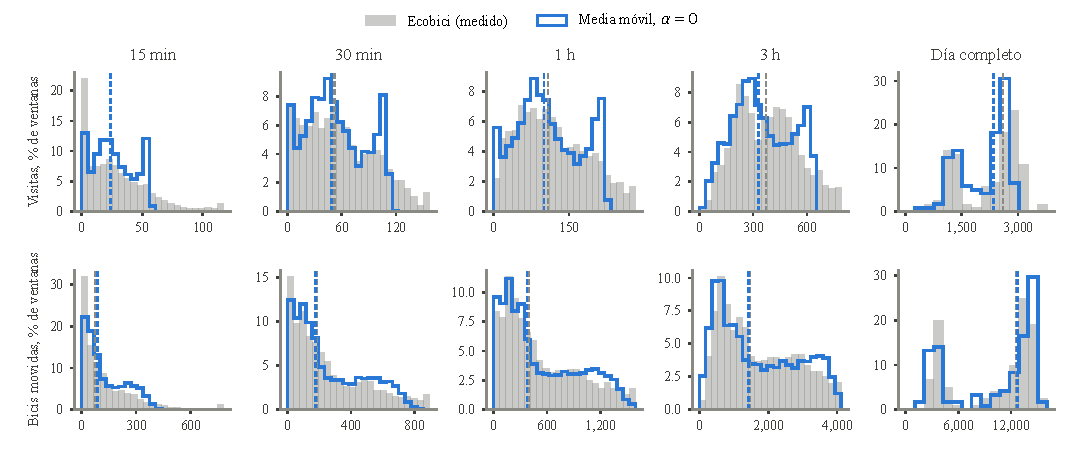
\includegraphics[width=\textwidth]{figs/caso-ritmo.pdf}
\caption{Ritmo del rebalanceo en los \rtDias{} días de prueba: visitas (arriba) y bicis movidas (abajo) aplicadas en ventanas móviles de 15 minutos a 3 horas y en el día completo. Gris: Ecobici medido; azul: media móvil con $\alpha=0$; líneas punteadas: medianas. En las ventanas móviles, la última barra incluye los valores mayores al percentil 99.5.}
\label{fig:ritmo}
\end{figure*}

\begin{table*}[!htb]
\centering\footnotesize
\setlength{\tabcolsep}{4pt}
\caption{Mediana, percentil 95 y máximo de visitas y bicis movidas por ventana en los \rtDias{} días de prueba. Eco.: Ecobici medido; MM: media móvil con $\alpha=0$.}
\label{tab:ritmo}
\begin{tabular}{@{}lrrrrrrrrrrrr@{}}
\toprule
 & \multicolumn{6}{c}{Visitas} & \multicolumn{6}{c}{Bicis movidas} \\
\cmidrule(lr){2-7}\cmidrule(l){8-13}
 & \multicolumn{2}{c}{Mediana} & \multicolumn{2}{c}{p95} & \multicolumn{2}{c}{Máximo} & \multicolumn{2}{c}{Mediana} & \multicolumn{2}{c}{p95} & \multicolumn{2}{c}{Máximo} \\
Ventana & Eco. & MM & Eco. & MM & Eco. & MM & Eco. & MM & Eco. & MM & Eco. & MM \\
\midrule
15 min & 24 & 24 & 78 & 54 & 246 & 61 & 75 & 88 & 436 & 338 & 1,325 & 465 \\
30 min & 52 & 49 & 127 & 108 & 346 & 117 & 186 & 178 & 751 & 671 & 1,446 & 857 \\
1 h & 108 & 100 & 243 & 213 & 621 & 228 & 399 & 373 & 1,378 & 1,330 & 2,017 & 1,646 \\
3 h & 372 & 329 & 688 & 614 & 1,390 & 651 & 1,454 & 1,419 & 3,676 & 3,697 & 5,020 & 4,404 \\
Día completo & 2,596 & 2,341 & 3,183 & 2,784 & 3,776 & 2,973 & 12,625 & 12,729 & 14,702 & 14,915 & 15,551 & 16,090 \\
\bottomrule
\end{tabular}

\end{table*}

\section{El 1 de septiembre de 2025}\label{ap:mapas}
\begin{figure}[h]
\centering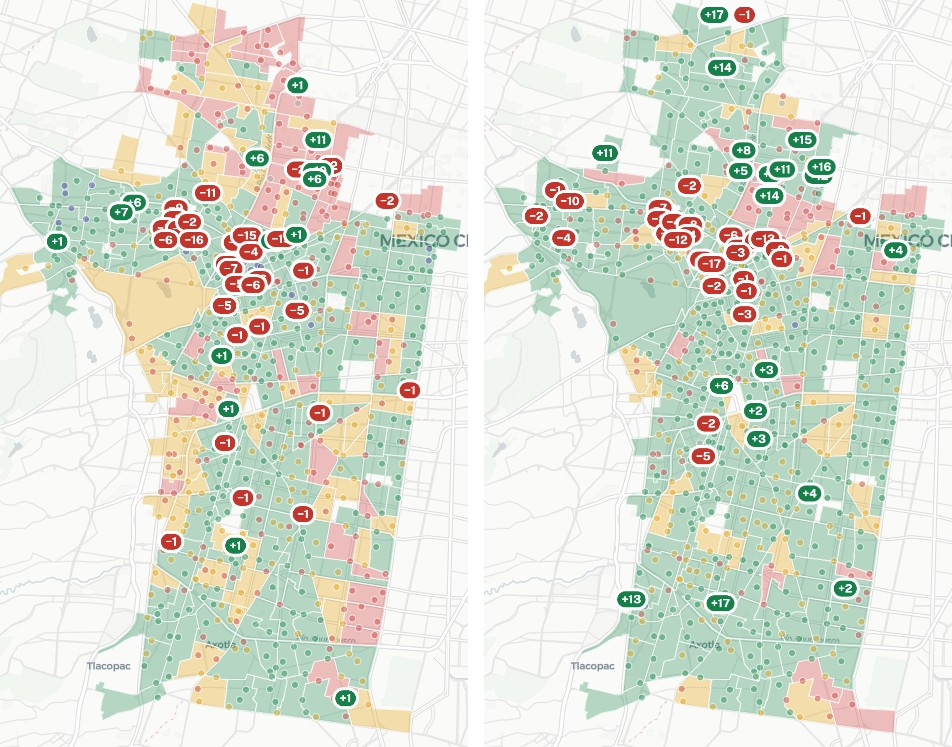
\includegraphics[width=\columnwidth]{figs/app-caso/eco-lgbm-0900-col.jpg}
\caption{Replay del \rejDia{} a las 9:00 en nuestra aplicación: Ecobici medido (izquierda) y LightGBM directo (derecha). Mismos colores que la Fig.~\ref{fig:sin}; las etiquetas $+N$ y $-N$ son las bicis entregadas y recogidas en esa foto.}
\label{fig:nueve}
\end{figure}

La Fig.~\ref{fig:veintiuno} es la comparación de la Fig.~\ref{fig:nueve} a las 21:00, la Tabla~\ref{tab:dia} da el día completo de las capturas y la Fig.~\ref{fig:sinlgbm} compara LightGBM directo con no rebalancear; entre las 8:45 y las 9:00 son \csBaseNueveEF{} contra \csLgbmNueveEF{} minutos-estación vacíos o llenos, y \csBaseNueveDesv{} contra \csLgbmNueveDesv{} desvíos.

\begin{figure}[h]
\centering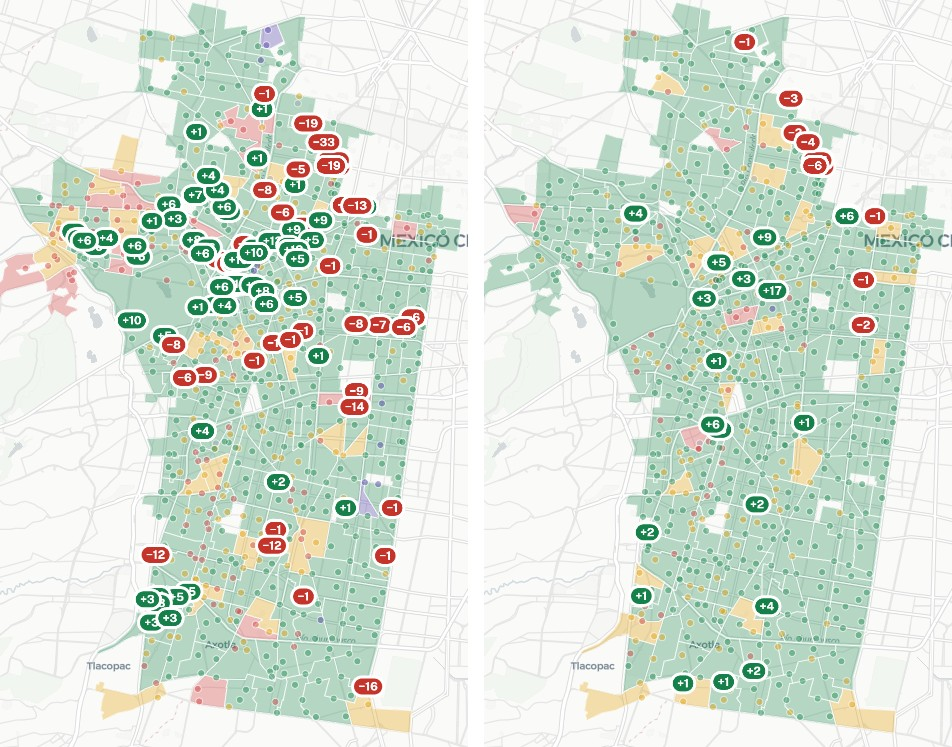
\includegraphics[width=\columnwidth]{figs/app-caso/eco-lgbm-2100-col.jpg}
\caption{Replay del \rejDia{} a las 21:00: Ecobici medido (izquierda) y LightGBM directo (derecha).}
\label{fig:veintiuno}
\end{figure}

\begin{table}[h]
\centering\footnotesize
\setlength{\tabcolsep}{4pt}
\caption{El \rejDia, día completo. Mismas unidades que la Tabla~\ref{tab:principal}; desvíos por día.}
\label{tab:dia}
\begin{tabular}{@{}lrrrrr@{}}
\toprule
Brazo & E & F & E+F & Desvíos & m/desv. \\
\midrule
Sin rebalanceo & 229,597 & 59,285 & 288,882 & 20,452 & 426 \\
Ecobici (medido) & 106,451 & 12,316 & 118,767 & 3,343 & 279 \\
LightGBM directo & 69,037 & 2,125 & 71,162 & 5,517 & 263 \\
Oráculo directo & 36,227 & 851 & 37,078 & 2,922 & 257 \\
\bottomrule
\end{tabular}

\end{table}

\begin{figure*}[h]
\centering
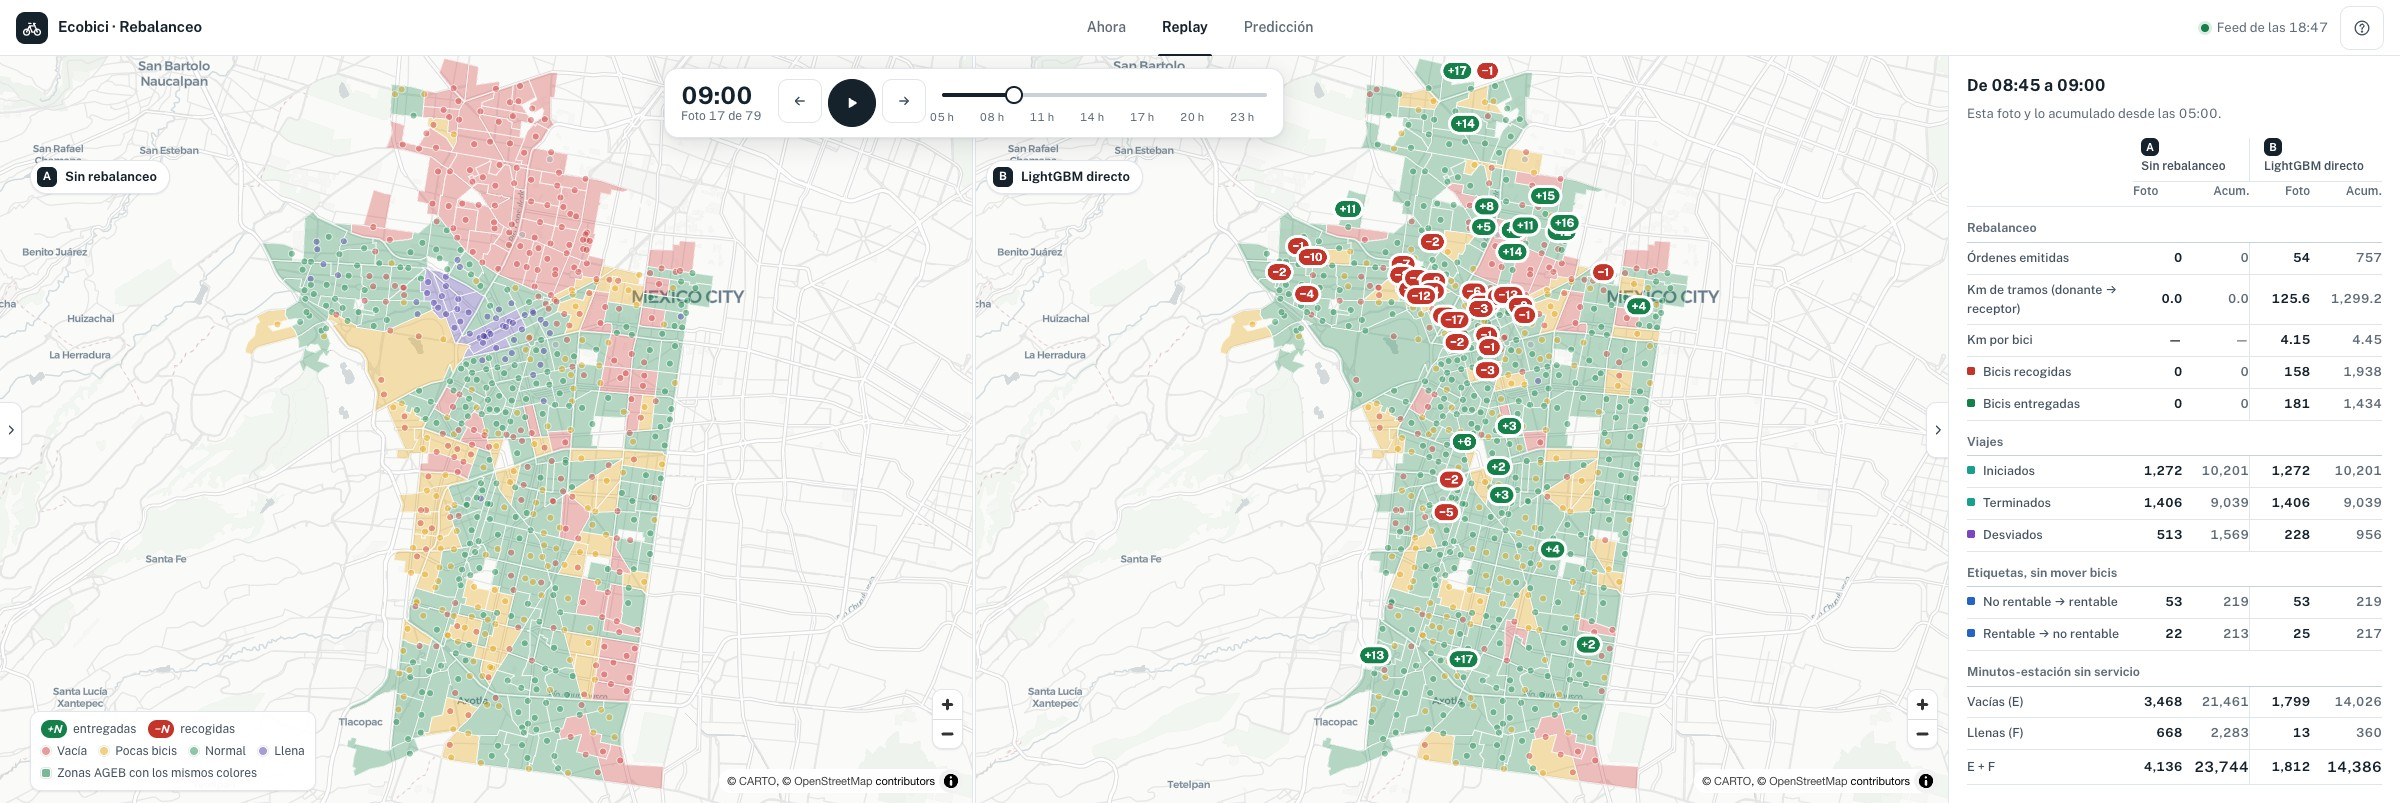
\includegraphics[width=\textwidth]{figs/app-caso/sin-lgbm-0900.jpg}\\[2pt]
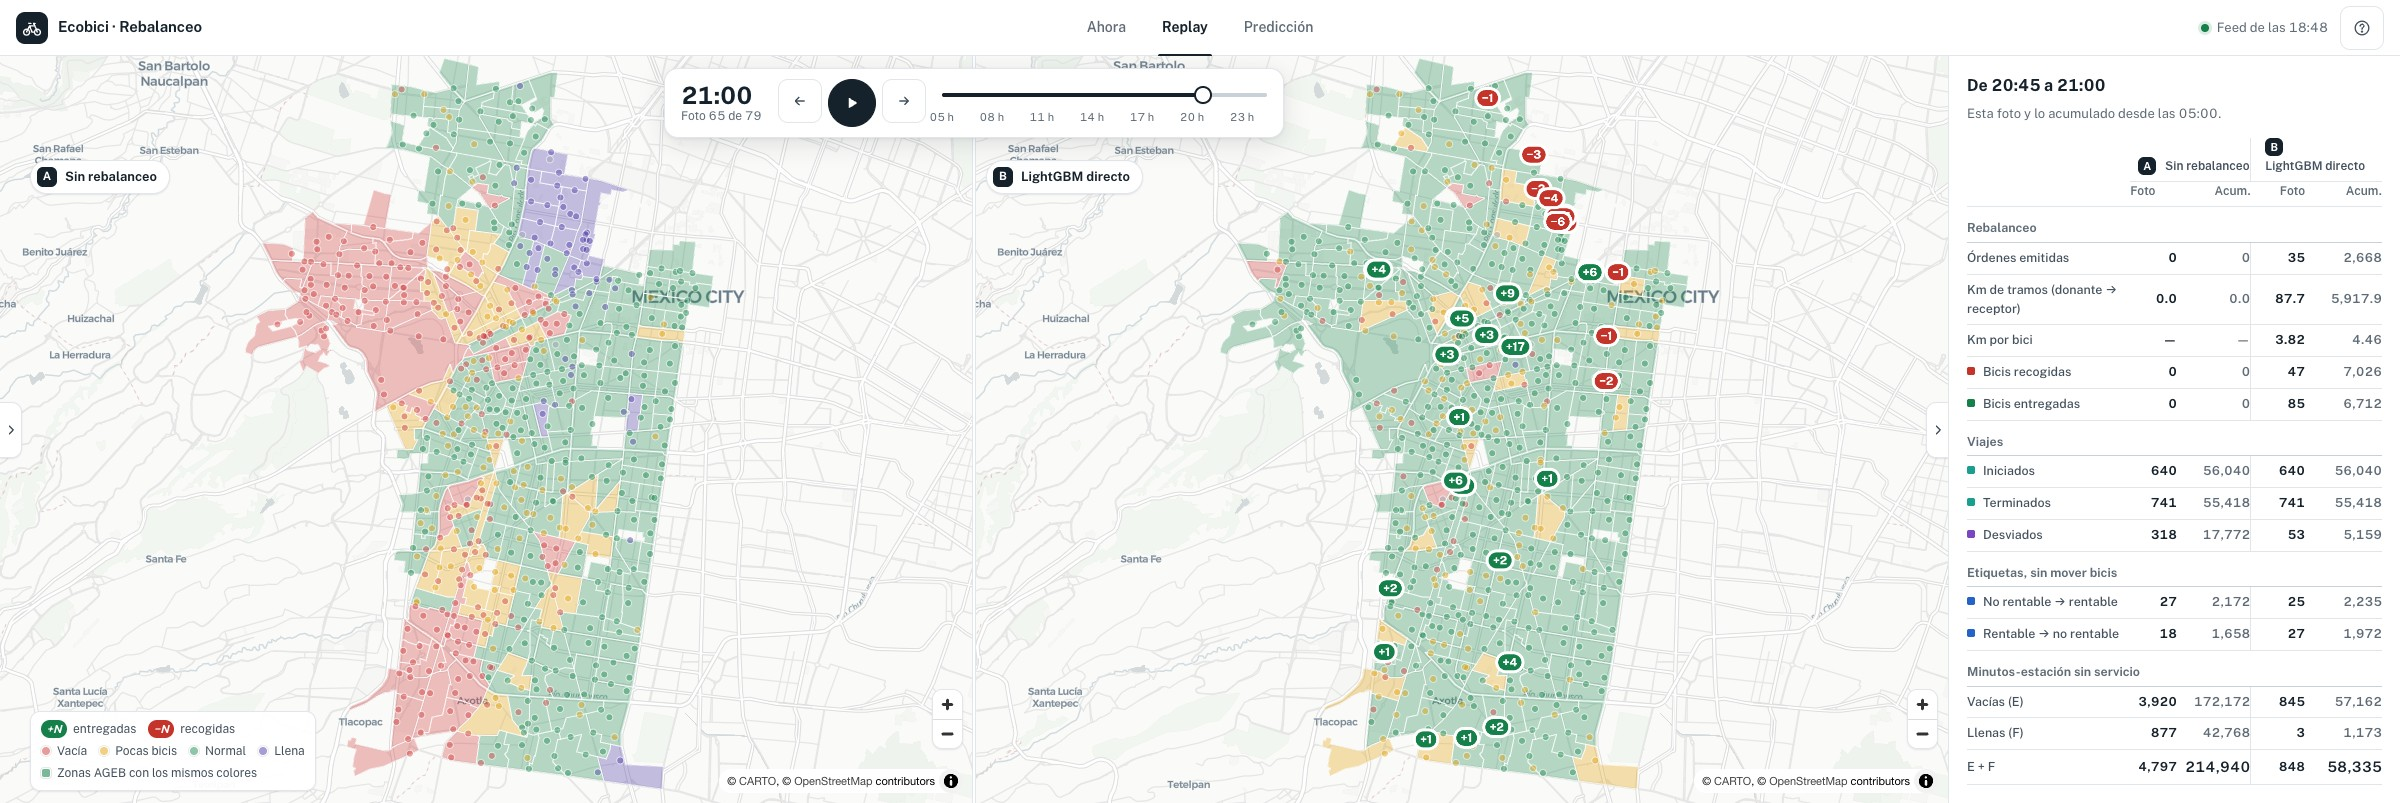
\includegraphics[width=\textwidth]{figs/app-caso/sin-lgbm-2100.jpg}
\caption{Replay del \rejDia: sin rebalanceo (A) contra LightGBM directo (B), a las 9:00 (arriba) y a las 21:00 (abajo), con el cuadre de cada foto a la derecha.}
\label{fig:sinlgbm}
\end{figure*}

\section{Rebalanceo de Ecobici, bodega, no rentables y exactitud}\label{ap:ecobici}
Los datos indican que Ecobici rebalancea siguiendo a la demanda con un pequeño retraso, como se ve en la Fig.~\ref{fig:hora}.

\begin{figure}[h]
\centering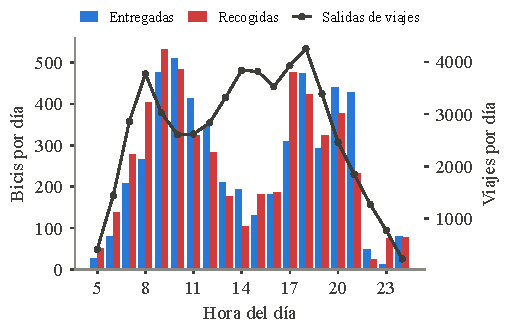
\includegraphics[width=\columnwidth]{figs/caso-por-hora.pdf}
\caption{Bicis que entrega y recoge Ecobici por hora (eje izquierdo) y salidas de viajes (eje derecho), media de \rdias{} días. Movimientos medidos con la ecuación~\eqref{eq:delta}, sin pares, a la hora de la segunda foto. La hora 24 va de 00:00 a 00:30.}
\label{fig:hora}
\end{figure}

Hay dos olas. La de la mañana alcanza su máximo a las \chPicoHora, con unas \chPicoBicis{} bicis movidas por día en esa hora, justo después del pico de viajes de las 8:00; la de la tarde se extiende de las 17:00 a las 21:00. Entre las 6:00 y las 10:00 se mueve el \chMananaPct\% de las bicis y entre las 16:00 y las 21:00 el \chTardePct\%, mientras que al mediodía, pese a que hay muchos viajes, el rebalanceo es bajo. También hay rebalanceo nocturno, entre las 00:30 y las 05:00, que no simulamos porque cada día arranca con el estado de las 05:00.

\subsection{Bodega}
Las bicis se averían y se reparan, así que entran y salen del sistema a través de la bodega. Nuestros datos indican que, en el largo plazo, ese flujo neto es nulo, y lo verificamos de dos formas. Por identificadores, el número de bicis distintas que se usan cada día casi no cambia (en promedio \cbActivasSep{} en septiembre, \cbActivasOct{} en octubre y \cbActivasNov{} en noviembre de 2025), y en esos tres meses aparecen solo \cbIdsNuevos{} bicis que no habíamos visto antes. Por totales, entre las 04:30 y las 05:00 el sistema está cerrado y todas las bicis están ancladas, así que la foto más cercana a las 04:45 cuenta la flota completa en estaciones. De un día al siguiente ese total cambia en promedio \cbMedia{} bicis, con un IC95 de \cbLo{} a $+$\cbHi{} en \cbPares{} pares de días consecutivos: en el largo plazo, la diferencia es cero. 

\subsection{Bicis no rentables}
El feed distingue las bicis ancladas disponibles ($b$) de las no rentables ($d$). No rentable no significa descompuesta, porque el contador sube y baja todo el día: muchas bicis quedan bloqueadas un rato al llegar o se reportan con una falla que se repara ahí mismo. Un cambio de no rentable a rentable no es rebalanceo, ya que es la misma bici en la misma estación con otra etiqueta, y si lo contáramos como movimiento cada reporte de falla aparecería como una visita de Ecobici. Por eso la ecuación~\eqref{eq:delta} suma disponibles y no rentables, de modo que un cambio de etiqueta da cero, como muestra la Tabla~\ref{tab:etiqueta} del Apéndice~\ref{ap:auditoria} para una estación con cinco disponibles y dos no rentables, sin viajes de por medio.

En los \rdias{} días de prueba cambian de etiqueta unas \retiquetasDia{} bicis por día, y en el \renSitioPct\% de esos cambios el total de la estación no se altera. El simulador aplica cada cambio de etiqueta observado en la misma estación y a la misma hora para todas las políticas; una estación con cero disponibles y tres no rentables cuenta como vacía, y el asignador solo mueve bicis disponibles. El supuesto es conservador para nuestras políticas, porque en la realidad Ecobici puede llevarse una bici dañada y devolverla reparada donde le convenga.

\begin{table}[h]
\centering\footnotesize
\setlength{\tabcolsep}{3.5pt}
\caption{Exactitud de cada pronóstico en los \cfMeses{} meses de prueba, por estación y por hora. MAE en viajes; WAPE en porcentaje; neto: llegadas menos salidas.}
\label{tab:pron}
\begin{tabular}{@{}lrrrrrr@{}}
\toprule
 & \multicolumn{2}{c}{Salidas} & \multicolumn{2}{c}{Llegadas} & \multicolumn{2}{c}{Neto} \\
Pronóstico & MAE & WAPE, \% & MAE & WAPE, \% & MAE & WAPE, \% \\
\midrule
\multicolumn{7}{@{}l}{\emph{Primera hora}} \\
Media móvil & 1.59 & 40 & 1.53 & 39 & 1.62 & 82 \\
LightGBM diario & 1.57 & 40 & 1.50 & 38 & 1.60 & 81 \\
LightGBM directo & 1.79 & 45 & 1.69 & 43 & 1.99 & 88 \\
\midrule
\multicolumn{7}{@{}l}{\emph{Hora 4 hacia adelante}} \\
Media móvil & 1.67 & 40 & 1.62 & 39 & 1.68 & 86 \\
LightGBM diario & 1.64 & 40 & 1.59 & 38 & 1.66 & 85 \\
LightGBM directo & 1.89 & 46 & 1.83 & 43 & 2.05 & 91 \\
\bottomrule
\end{tabular}

\end{table}

\section{Ventanas de entrenamiento y prueba}\label{ap:ventanas}
\begin{figure}[h]
\centering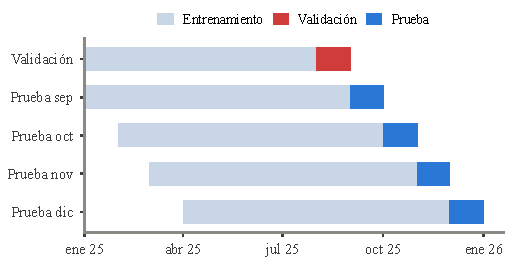
\includegraphics[width=\columnwidth]{figs/caso-ventanas.pdf}
\caption{Dónde entrenamos y dónde probamos. Cada fila es un mes evaluado: en gris claro, los meses con que se entrenan los LightGBM (siete para la validación de agosto, ocho para cada mes de prueba); en color, el mes evaluado. La media móvil solo usa las cuatro semanas previas a cada día.}
\label{fig:ventanas}
\end{figure}

Para elegir $n$ corrimos el asignador con los dos oráculos, que marcan hasta dónde puede llegar con información perfecta, con $n$ de 2 a \rnMax{} horas y $\lambda\in\{\rlamGridN\}$; $n=1$ equivale a no rebalancear. Para cada día promediamos $\EF$ sobre las tres $\lambda$ y, para $n=1,2,\dots$, calculamos el IC95 $t$ pareado por día de la diferencia entre $n+1$ y $n$. Nos quedamos con el primer $n$ cuyo siguiente no mejora de forma demostrable, es decir, cuyo límite superior es mayor o igual a cero: $n=\rnDiario$ para la forma diaria y $n=\rnDirecto$ para la directa.

Para elegir $\lambda$ y comparar con el mismo esfuerzo, buscamos para cada uno de los cinco brazos con asignador la $\lambda$ con la que hace tantas visitas por día como Ecobici en la validación, \rselEcoVis. Corrimos cada brazo con su $n$ en una rejilla de $\lambda$ de 10 a 120 minutos-estación; como las visitas bajan al subir $\lambda$, interpolamos linealmente entre los dos puntos que encierran el objetivo, corrimos la $\lambda$ resultante para confirmarla y la aceptamos si sus visitas quedaban a menos del 1\% del objetivo; si no, sumamos ese punto a la curva y repetimos. La confirmación tomó a lo más \rlamRondasMax{} rondas, y ningún brazo quedó a más del \rlamDifMax\% del objetivo. Quedaron \rlamMa{} para la media móvil, \rlamLgbmD{} y \rlamLgbmDir{} para los dos LightGBM, y \rlamOrD{} y \rlamOrDir{} para los oráculos.

\section{Cómo reproducir y uso de IA}\label{ap:repro}
El código, la aplicación y las instrucciones están en \cite{repo}. Todos los comandos se corren con \texttt{uv run} desde la raíz.

\begin{center}\footnotesize
\begin{tabularx}{\columnwidth}{@{}p{2.7cm}Y@{}}
\toprule
Qué & Comando (\texttt{uv run} \dots) \\
\midrule
Viajes y fotos & \texttt{python -m ecosim.data build-trips} y \texttt{build-snapshots} \\
Movimientos de Ecobici y topes & \texttt{python -m ecosim.medicion} \\
Pronósticos y exactitud & \texttt{python -m ecosim.pronostico} \\
Experimento & \texttt{python -m ecosim.run -{}-all} \\
Real contra simulado & \texttt{python3 report/figs/fidelidad\_ecobici.py} \\
Cifras y tablas & \texttt{python3 report/figs/numeros\_run3.py} y \texttt{figs\_caso.py} \\
Comprobar cifras & los tres, con \texttt{-{}-check} \\
\bottomrule
\end{tabularx}
\end{center}
Cada cifra del texto es una macro con su origen en \texttt{report/fuentes-numeros.md} y \texttt{report/figs/figs\_caso.json}.

Usamos asistentes de programación con IA generativa (Claude Code y Codex) para escribir y revisar código, correr los experimentos y redactar borradores de este texto. Las decisiones de planteamiento y de supuestos son nuestras, y ninguna cifra se escribió a mano: todas salen de los scripts de la tabla anterior.
\end{document}
